\documentclass[aspectratio=169]{beamer}
\usepackage{booktabs}
\usepackage{xcolor}
\usepackage{changepage}
\usepackage[export]{adjustbox}
\usepackage{booktabs}
\usepackage{graphbox}

\usetheme[numbering=fraction,progressbar=frametitle]{metropolis}


% Backup
\newcommand{\backupbegin}{%
   \newcounter{finalframe}
   \setcounter{finalframe}{\value{framenumber}}
}
\newcommand{\backupend}{%
   \setcounter{framenumber}{\value{finalframe}}
}


% Colors
\definecolor{myBlue}{RGB}{21, 56, 110}
\definecolor{myRed}{RGB}{174,0,34}
\definecolor{myRedBg}{RGB}{251, 217, 224}
\definecolor{greySAS}{RGB}{167,166,166}
\definecolor{greyCU}{RGB}{44,46,53}

\setbeamercolor{title}{fg=myBlue}
\setbeamercolor{background canvas}{bg=white}
\setbeamercolor{normal text}{fg=black}
\setbeamercolor{frametitle}{fg=myBlue, bg=white}
\setbeamercolor{section title}{fg=myBlue}
\setbeamercolor{title separator}{fg=myRed,bg=myRedBg}
\setbeamercolor{progress bar}{fg=myRed,bg=myRedBg}
\setbeamercolor{structure}{fg=myRed}


% Thicker progress bar
\makeatletter
\setlength{\metropolis@titleseparator@linewidth}{1pt}
\setlength{\metropolis@progressonsectionpage@linewidth}{1pt}
\setlength{\metropolis@progressinheadfoot@linewidth}{1pt}
\makeatother


% Commands
\newcommand{\bluetext}[1]{%
  \textcolor{myBlue}{#1}
}
\newcommand{\redtext}[1]{%
  \textcolor{myRed}{#1}
}


% Variables
\def\pt{\ensuremath{p_\mathrm{T}}}


% Title
\title[FCCcalo]{Calorimetry for Future Circular Collider}
\author[Faltova, Smiesko]{Jana~Faltov\'{a}\inst{1}, Juraj~Smie\v{s}ko\inst{1,2}}
\institute[CU, SAS]{\inst{1} Charles University, Czechia \\
                    \inst{2} Slovak Academy of Sciences, Slovakia}
\date[2021-May-19]{\footnotesize
                   IPNP Seminar, Prague \\
                   19 May 2020}
\titlegraphic{\vspace{6.1cm}
  \begin{center}
    
\includegraphics[align=c, width=0.2\linewidth]{figures/Logo_AIDAinnova.png}
    %\vspace{5em}
    
\includegraphics[align=c, width=0.6\linewidth]{figures/logolink_OP_VVV_hor_barva_eng.jpg}
  \end{center}
}

%
% -----------------------------------------------------------------------------
%
\begin{document}

{%
  \setbeamercolor{background canvas}{bg=greyCU}
  \begin{frame}[noframenumbering]
    \centering
    \vspace{1cm}
    
\includegraphics[width=.25\textwidth]{figures/CU_red_white_logo.pdf}
    \thispagestyle{empty}
  \end{frame}
}

\begin{frame}
  \titlepage{}
  \thispagestyle{empty}
\end{frame}


\begin{frame}
  \frametitle{Overview}

  \tableofcontents
\end{frame}

%
% -----------------------------------------------------------------------------
%
\begin{frame}
  \frametitle{Questionnaire}

  \begin{columns}
    \column{.7\textwidth}

    \begin{itemize}
      \item Are you a fan of new large scale experiments in HEP\@?
      \item Are you interested in the progress of the FCC project?
      \item Would you like to join the preparatory face of the experiment?
      \item Are you interested in R\&D projects or hardware?
      \item Would you like to know what Juraj and myself are working on?
    \end{itemize}

    \column{.3\textwidth}

    \begin{center}
      
\includegraphics[width=0.5\linewidth]{figures/question.png}
    \end{center}
  \end{columns}
  \pause%

  \vspace{1ex}
  \bluetext{If you answered at least once ``YES'', you're certainly\\ interested
            in the topic of this talk!}
  \pause%

  \vspace{-3ex}
  \begin{columns}
    \column{.7\textwidth}

    \bluetext{\bf If your interest still remains after the talk, do not
              hesitate to contact us :)}

    \column{.3\textwidth}

    \vspace{-3ex}
    \begin{center}
      
\includegraphics[width=0.8\linewidth]{figures/weWantYou.png}\\
    \end{center}
  \end{columns}
\end{frame}

\section{Future Colliders}

\begin{frame}
  \frametitle{Future Colliders}

  \begin{columns}[c]
    \column{.4\textwidth}

    \bluetext{Large Hadron Collider at CERN}
    \begin{itemize}
    \item LHC (2008--2024)\\
     8--13~TeV, 400 fb$^{-1}$
    \item HL-LHL (2027--2040)\\
     14~TeV, 4000 fb$^{-1}$
    \end{itemize}

    \column{.6\textwidth}

    \begin{center}
      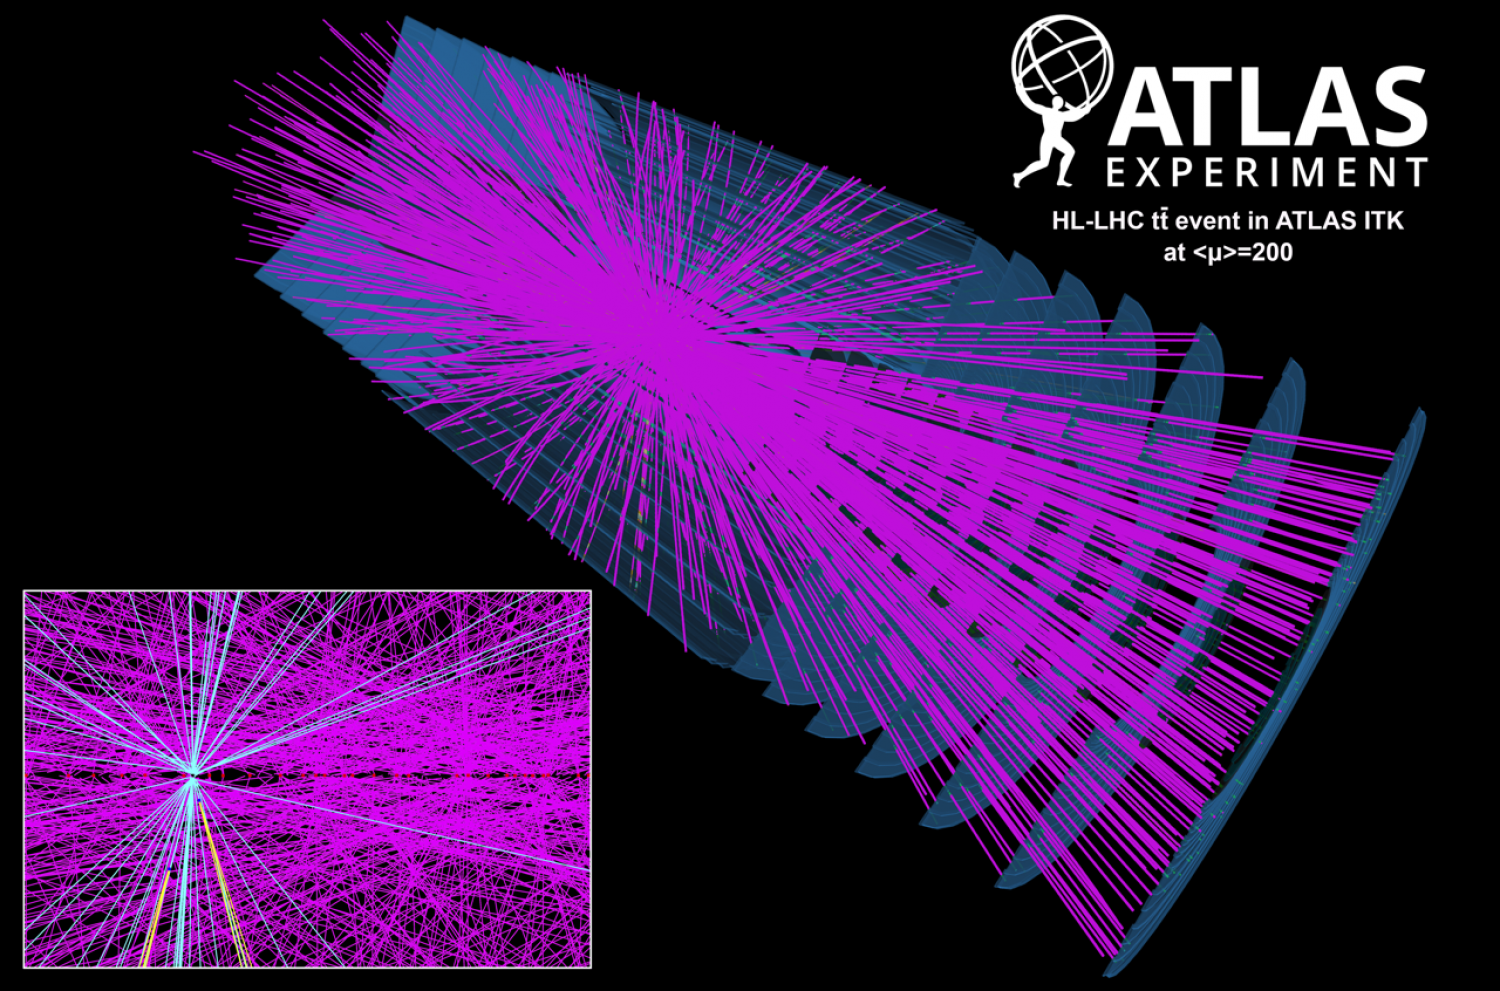
\includegraphics[width=0.75\linewidth]{figures/HL-LHC-tt.png} \\
    \end{center}
  \end{columns}
  \pause%

  \vspace{2ex}
  \bluetext{{\bf Next generation of colliders after LHC era?}} \\
  \vspace{2ex}

  \bluetext{European Strategy of Particle Physics 2020} \\
  \begin{itemize}
    \item New $e^+e^-$ collider (Higgs factory) as the highest-priority
    \item Hadron collider with $E_{\mathrm{cms}}$ at least 100 TeV at CERN as
          a longer term
  \end{itemize}
\end{frame}


\begin{frame}
  \frametitle{Why do we need new hadron collider?}

  \begin{columns}[c]
    \column{.6\textwidth}

    \bluetext{{\bf Hadron collider as a discovery machine}}\\
    % \vspace{2ex}

    \bluetext{Open questions}
    \begin{itemize}
      \item Dark matter
      \item Matter-antimatter symmetry
      \item Neutrino masses
      \item \dots
    \end{itemize}
    \pause%

    \bluetext{Hadron collider can give answers if}
    \begin{itemize}
      \item Mass of new particles is in its reach
      \item The detectors are sensitive enough
    \end{itemize}

    \column{.4\textwidth}

    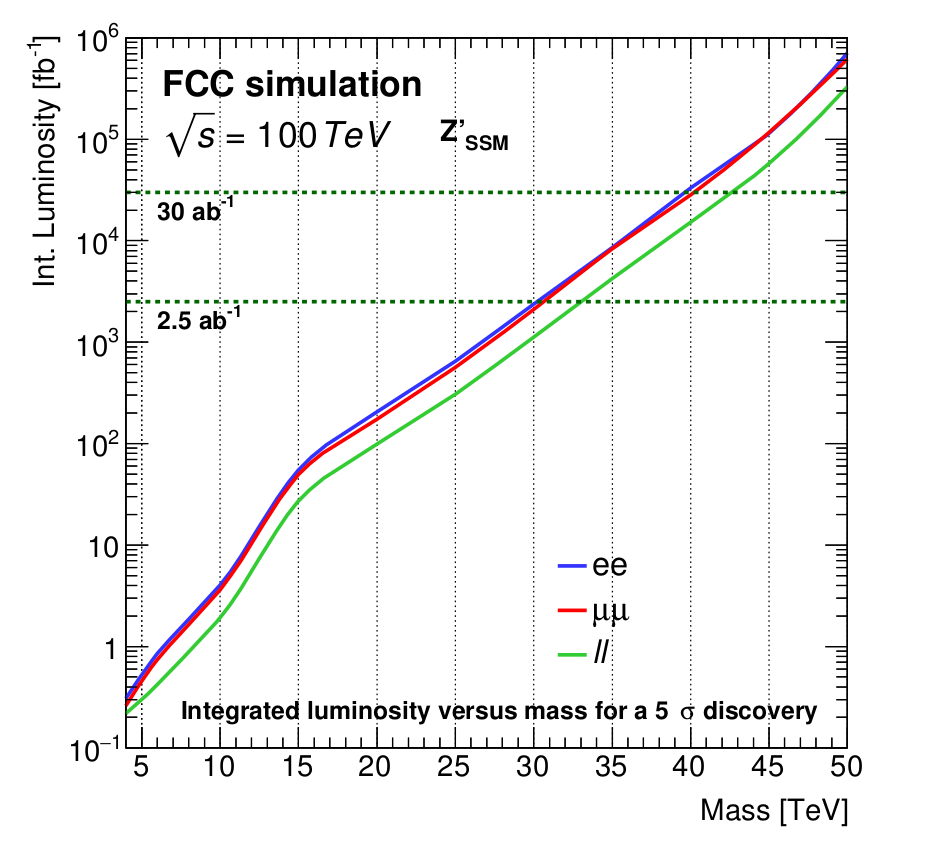
\includegraphics[width=\linewidth]{figures/zprime-search-fcchh.png} \\
    \tiny{Image: \href{https://cds.cern.ch/record/2651300?ln=en}{FCC-hh CDR}}
  \end{columns}
\end{frame}


\begin{frame}
  \frametitle{Why do we need new lepton collider?}
  
 \vspace{2ex}
 \begin{columns}[c]
    \column{.5\textwidth}
  \bluetext{{\bf Precise measurements of the electroweak sector as a hint
  of new physics}} \\[2ex]

  \bluetext{Highlights from the physics programme}
  \begin{itemize}
    \item Higgs boson couplings
    \item Top quark and Higgs boson masses
    \item Flavour physics ($b$, $c$, $\tau$)
  \end{itemize}

  \column{.5\textwidth}
    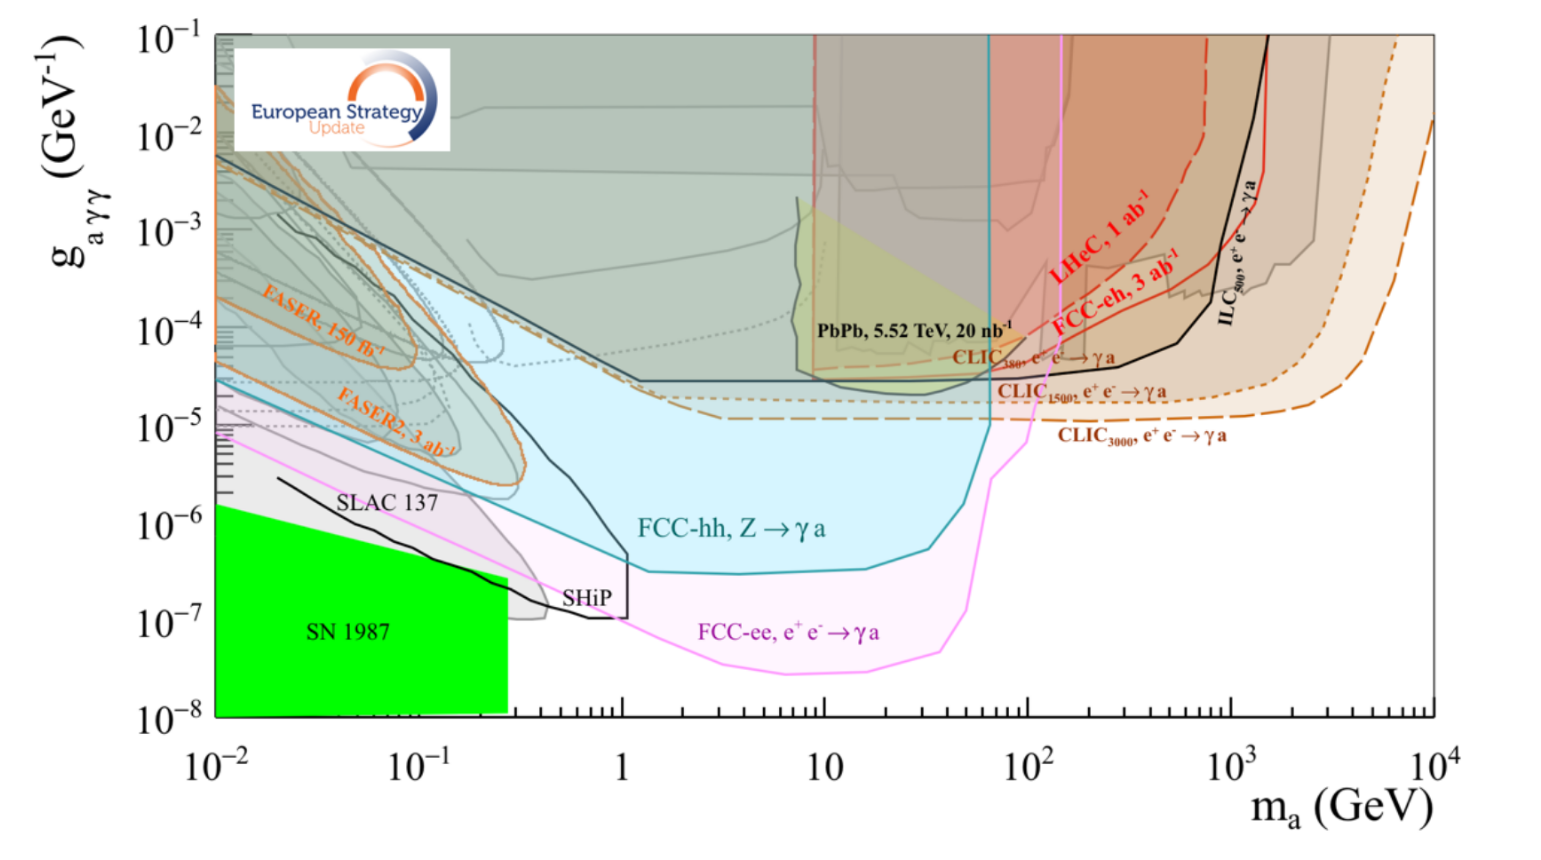
\includegraphics[width=\linewidth]{figures/axions.png} \\
    \tiny{Image: \href{https://arxiv.org/abs/1910.11775}{arXiv:1910.11775}}
  \end{columns}
 \pause%
 
  \vspace{1ex}
  \bluetext{Advantages of $e^+e^-$ colliders}
  \begin{itemize}
    \item Clean environment $\rightarrow$ measurements of unprecedented precision\\
    \item Higgs factories provides model-independent measurements
    \item We can starting building the collider (almost) now
  \end{itemize}
\end{frame}


\begin{frame}
  \frametitle{Lepton colliders at the market}

  \begin{columns}[c]
    \column{.7\textwidth}
    \bluetext{Linear Colliders}
    \begin{itemize}
      \item ILC (International Linear Collider, Japan)
      \item CLIC (Compact Linear Collider, CERN)
    \end{itemize}
    \bluetext{Circular Colliders}
     \begin{itemize}
     \item FCC (Future Circular Collider, CERN)
     \item CEPC (Circular Electron Positron Collider, China)
     \end{itemize}

    \column{.3\textwidth}
    
\includegraphics[width=0.4\linewidth]{figures/ilc_logo_400x400.jpg}\\
    \vspace*{-0.5cm}\hspace*{2cm}
\includegraphics[width=0.4\linewidth]{figures/CLIC-Logo-Color-72_3_0.png}\\
    
\includegraphics[width=0.6\linewidth]{figures/fcc_logo.jpg}\\
    \vspace*{-0.1cm}\hspace*{1.5cm}
\includegraphics[width=0.6\linewidth]{figures/cepc-logo.png}\\
   \end{columns}
\end{frame}


\begin{frame}
  \frametitle{Circular vs linear colliders}

  \begin{center}
    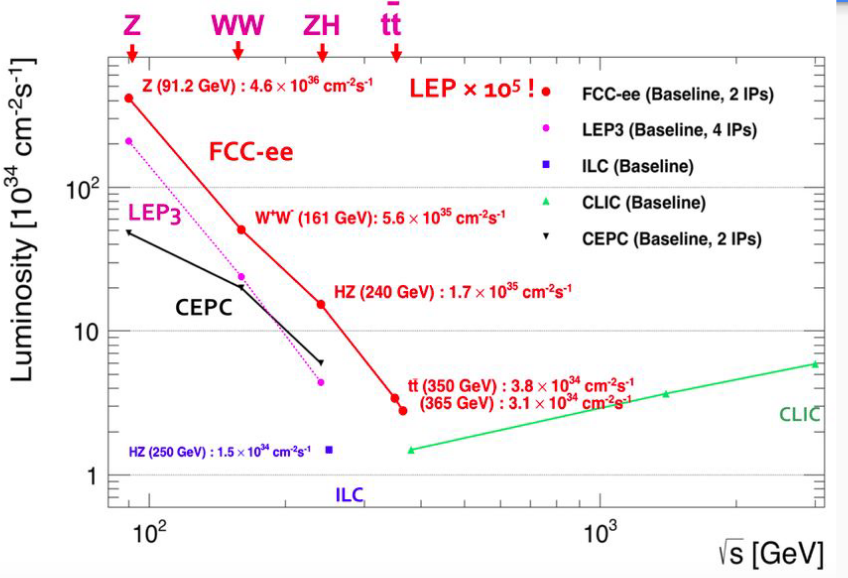
\includegraphics[width=0.4\linewidth]{figures/Luminosity_vs_energy_v1.png}\\
     \tiny{Image: \href{https://cds.cern.ch/record/2651299?ln=en}{FCC-ee CDR}}
  \end{center}
  \vspace{1ex}

  \begin{columns}
     \column{.4\textwidth}
     \bluetext{Linear colliders}
     \begin{itemize}
     \item High energy (extendable)
     \item No synchrotron radiation
     \item Beams not reusable
     \end{itemize}

     \column{.5\textwidth} 
     \bluetext{Circular colliders}
     \begin{itemize}
     \item High luminosity
     \item Synchrotron radiation
     \item Circulating beams
     \item Synergy with future $pp$ collider
     \end{itemize}
   \end{columns}
\end{frame}


\begin{frame}
  \frametitle{Higgs factories: Higgs coupling}
  \begin{center}
    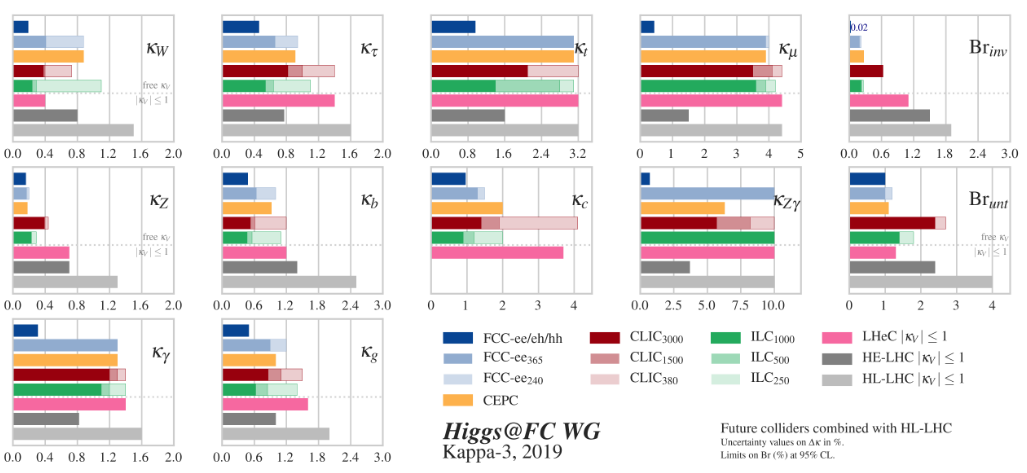
\includegraphics[width=0.85\linewidth]{figures/kappa.png}\\
    \tiny{Image: \href{https://arxiv.org/abs/1905.03764}{arXiv:1905.03764}}
  \end{center}
  \pause%

  %\small{
  Factor 2--10 improvement with $e^+e^-$ colliders wrt HL-LHC\\
  Comparable sensitivities in initial stages of $e^+e^-$ colliders (factor of 2 max)
  %}
\end{frame}


\begin{frame}
  \frametitle{Higgs factories: Higgs self-coupling}

  \begin{center}
    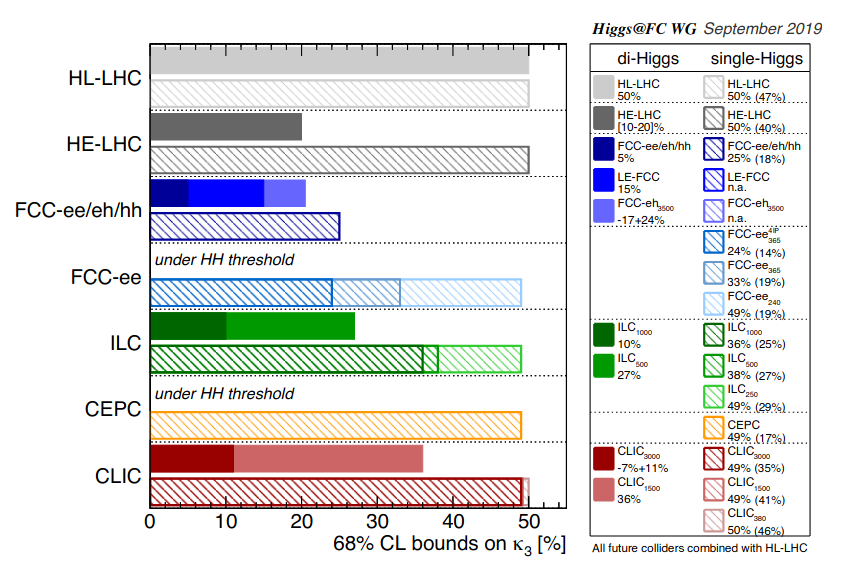
\includegraphics[width=0.6\linewidth]{figures/higgs_selfCoupling.png}\\
    \tiny{Image: \href{https://arxiv.org/abs/1905.03764}{arXiv:1905.03764}}
  \end{center}
  \pause

  A Higgs factory is needed, even if the ultimate goal is the hadron-hadron collider.\\
\end{frame}


\begin{frame}
  \frametitle{Possible timelines}
  \begin{center}
    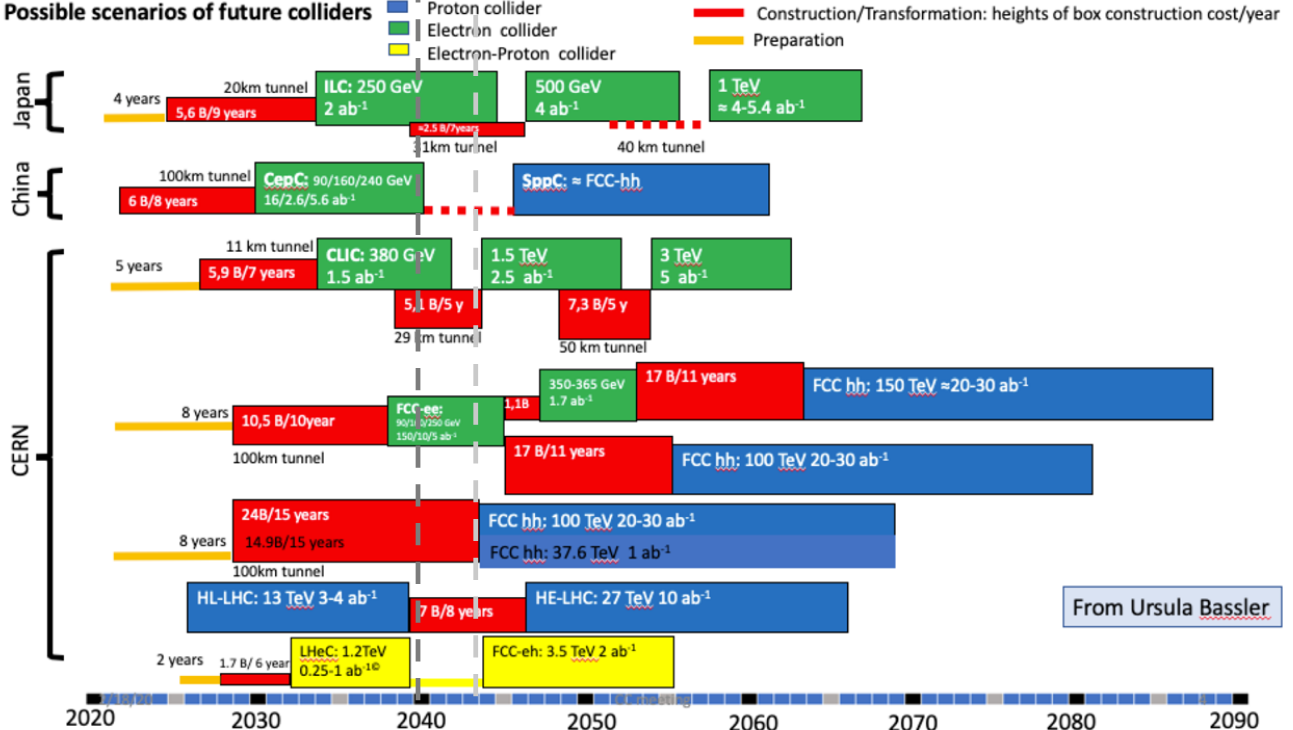
\includegraphics[width=0.8\linewidth]{figures/timeline-EPPSU2020.png}\\
  \end{center}
\end{frame}

%
% -----------------------------------------------------------------------------
%
\section{FCC Collider}

\begin{frame}
  \frametitle{Future Circular Collider}
  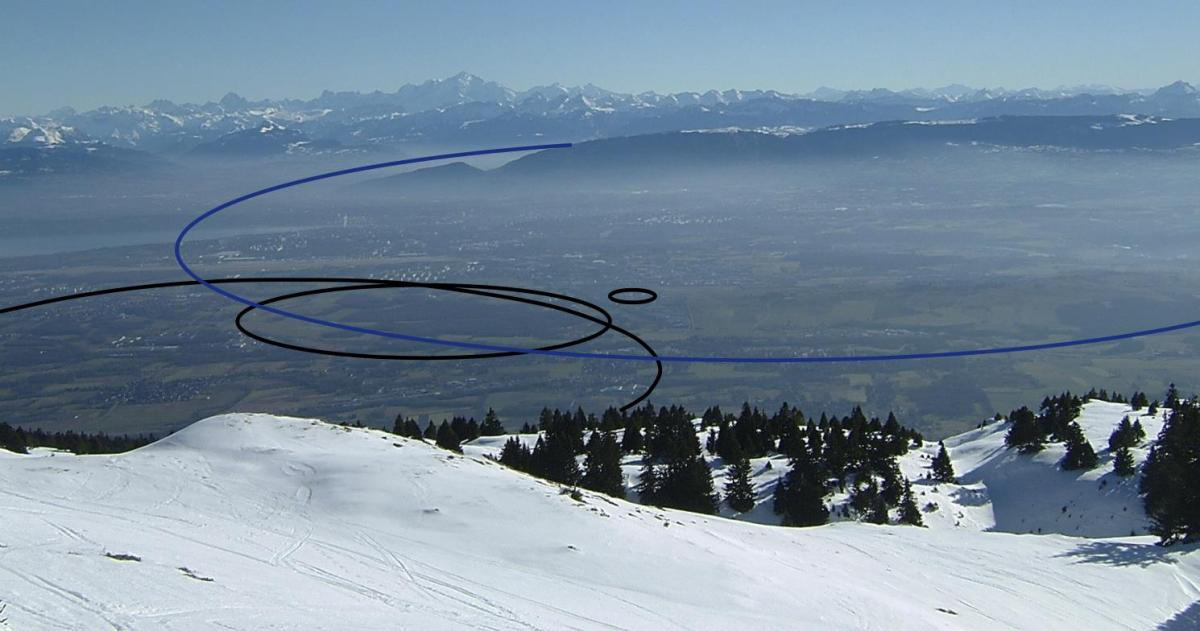
\includegraphics[width=1.0\linewidth]{figures/FCC_landscape.jpg}\\
\end{frame}

\begin{frame}
  \frametitle{FCC}

  \begin{center}
     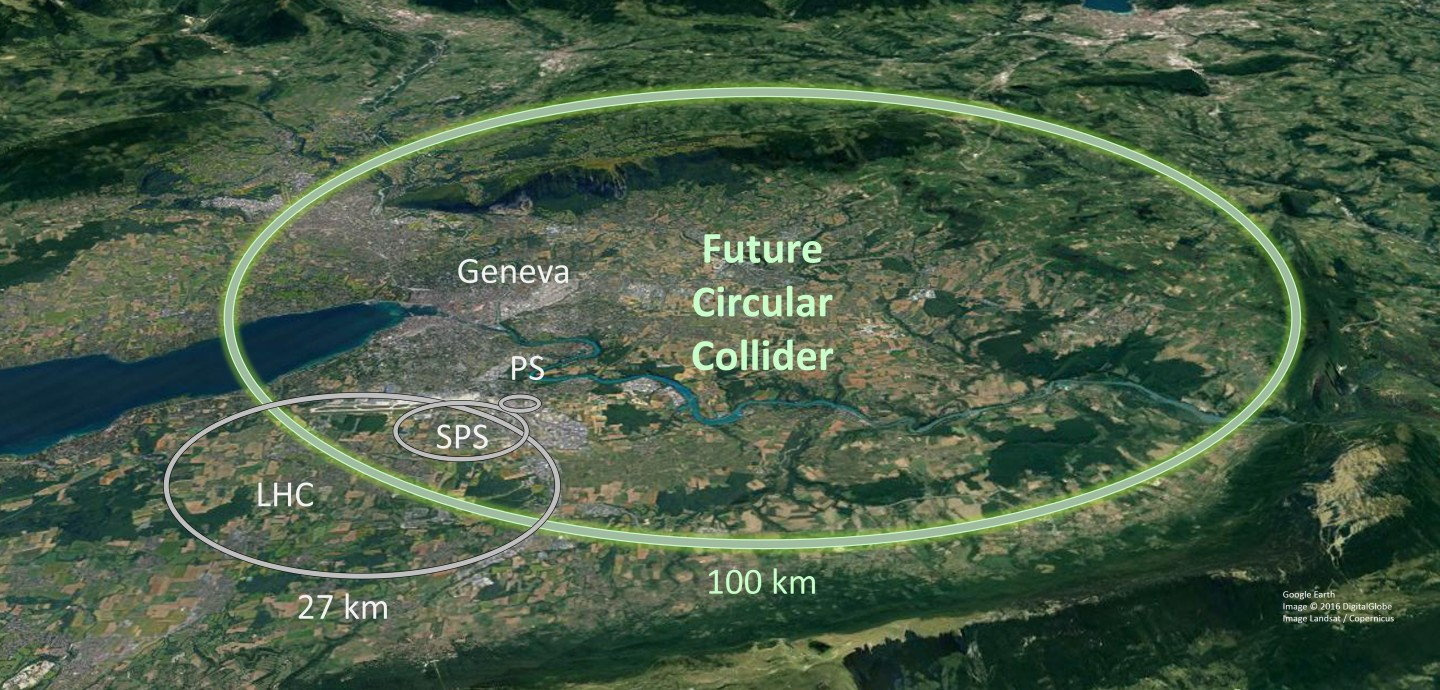
\includegraphics[width=0.6\linewidth]{figures/CERN-FCC.jpg}\\
  \end{center}

  \bluetext{{\bf Stage 1:} FCC-ee as Higgs factory, electroweak and top factory at highest luminosities}\\
  \bluetext{{\bf Stage 2:} FCC-hh (100 TeV) as a natural continuation, with ion and $eh$ option}\\
Complementary physics, common civil engineering and technical infrastructres\\
Building on and reusing CERN’s existing infrastructures\\

\end{frame}

\begin{frame}
  \frametitle{FCC-ee: Lepton collider}
  \begin{columns}[c]
     \column{.5\textwidth}
     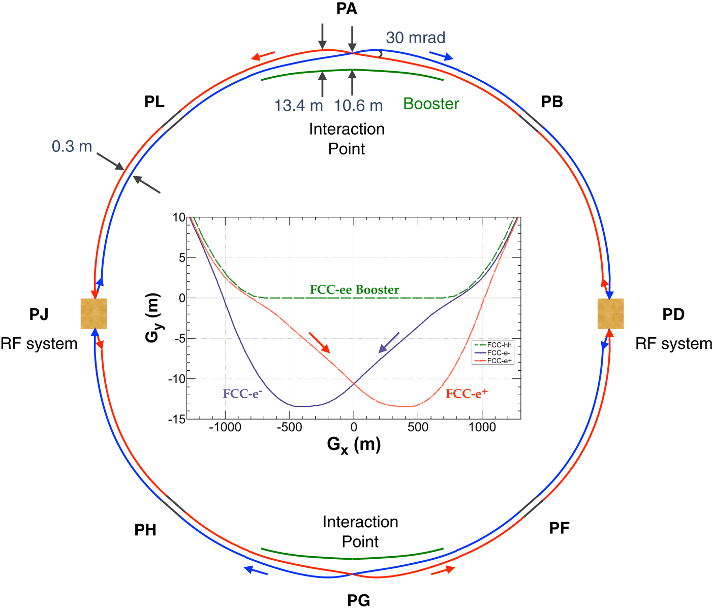
\includegraphics[width=0.8\linewidth]{figures/FCC_ee_ring.png}\\
     Double ring $e^+e^-$ collider (100 km)\\
     Asymmetric IR layout \& optics to limit synchrotron radiation\\
     \column{.5\textwidth}

     \begin{center}
       {\footnotesize\hspace{3.3em}88--95
                  \hspace{0.2em}\textcolor{blue}{158--162}
                  \hspace{0.2em}\textcolor{red}{240
                  }\hspace{1.9em}\textcolor{green}{345--365} GeV}
      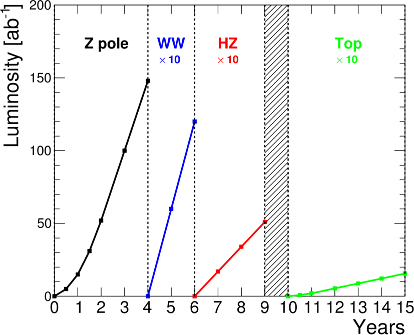
\includegraphics[width=.85\linewidth]{figures/FCC_ee_operation_plan.png}
     \end{center}
     Four working points\\
     $10^5 \times$ more $Z$ bosons compared to LEP\\
  \end{columns}
\end{frame}

\begin{frame}
    \frametitle{FCC-ee: Parameters}
    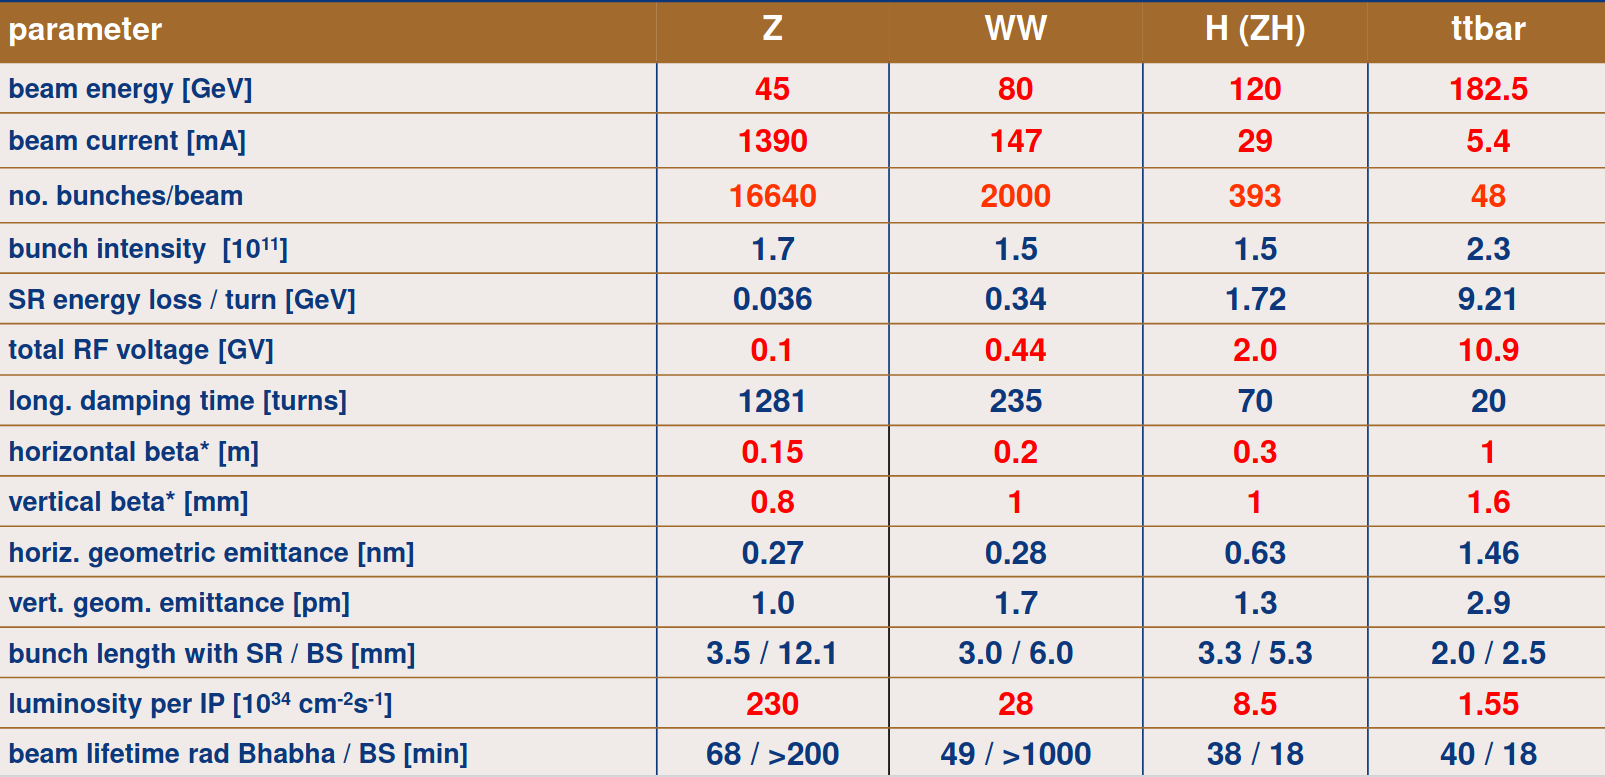
\includegraphics[width=1.0\linewidth]{figures/parameters-fccee.png}
\end{frame}


\begin{frame}
  \frametitle{FCC-ee: Key technologies}
  \begin{columns}[c]
    \column{.5\textwidth}

    \begin{center}
      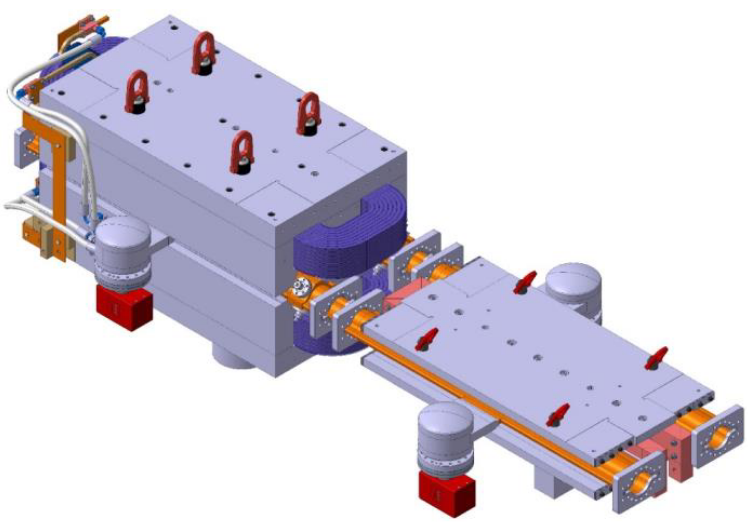
\includegraphics[width=0.6\linewidth]{figures/vacuumArc.png}\\
    \end{center}

    FCC-ee complete vacuum arc half-cell mock up\\[1ex]
    \small{%
    including girder, vacuum system with antechamber + pumps,
    dipole, quadrupole + sext.\ magnets, BPMs, cooling + alignment
    systems, technical infrastructure interfaces}

    \column{.5\textwidth}

    \begin{center}
      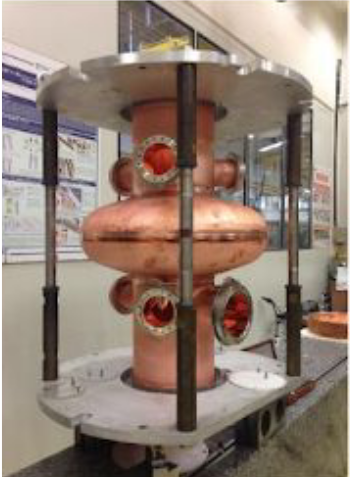
\includegraphics[width=0.35\linewidth]{figures/srfCavities.png}\\
    \end{center}

    \begin{itemize}
      \item 400 MHz SRF cryomodule
      \item Prototype multi-cell cavities for FCC $ZH$ operation
      \item High-efficiency RF power sources
    \end{itemize}
  \end{columns}
\end{frame}


\begin{frame}
  \frametitle{FCC-hh: Hadron collider}
   \begin{columns}[c]
    \column{.4\textwidth}
     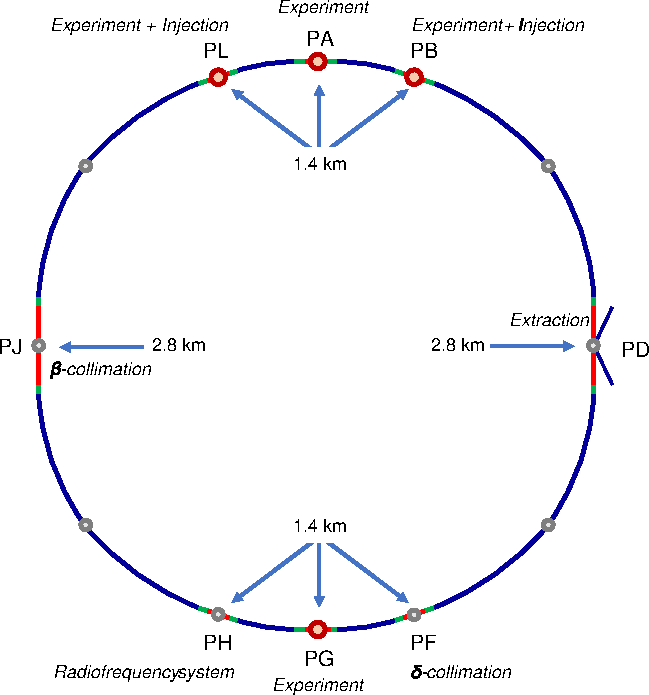
\includegraphics[width=1.0\linewidth]{figures/FCC_hh_ring.pdf}\\

     \column{.6\textwidth}
      \bluetext{Order of magnitude increase wrt HL-LHC}
      \begin{itemize}
      \item Centre of mass energy: 14 TeV $\rightarrow$ 100 TeV
      \item Total integrated luminosity: 4 ab$^{-1} \rightarrow$ 20 ab$^{-1}$
      \end{itemize}

      \bluetext{Key technology: 16 T dipole magnets}
      %\vspace{1ex}
      \begin{center}
        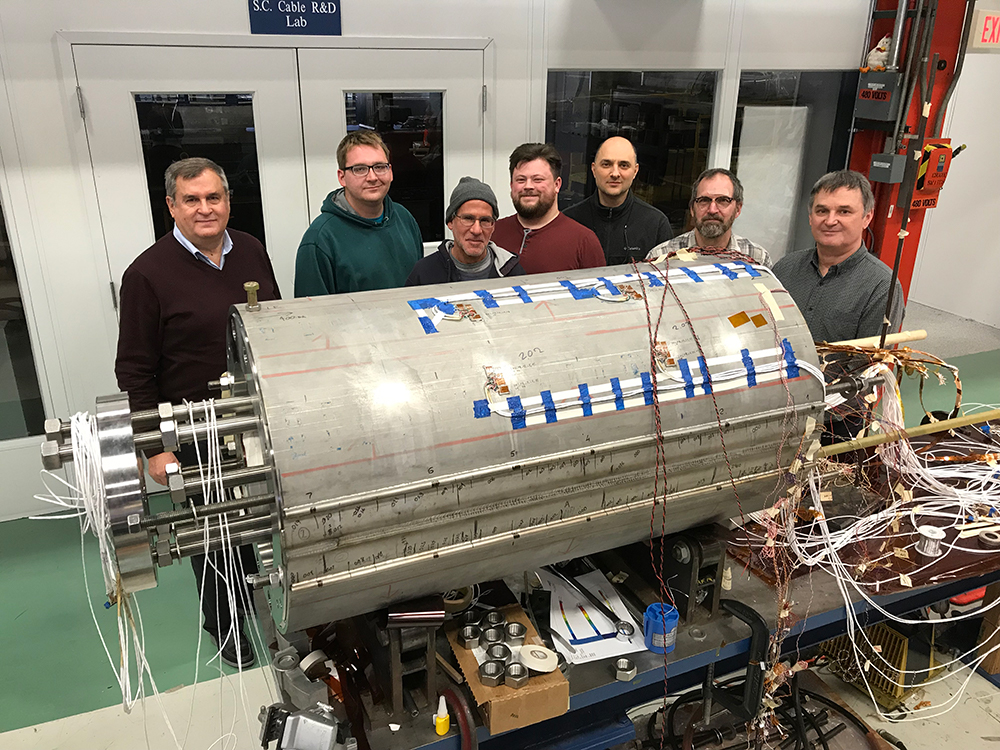
\includegraphics[width=.45\linewidth]{figures/fermilab-magnets-newdipole-small.jpg}\\
         {\small{Fermilab: Prototype of 14.1 T Nb$_3$Sn dipole magnet}}
       \end{center}
   \end{columns}
\end{frame}


\begin{frame}
  \frametitle{FCC-hh: parameters}
     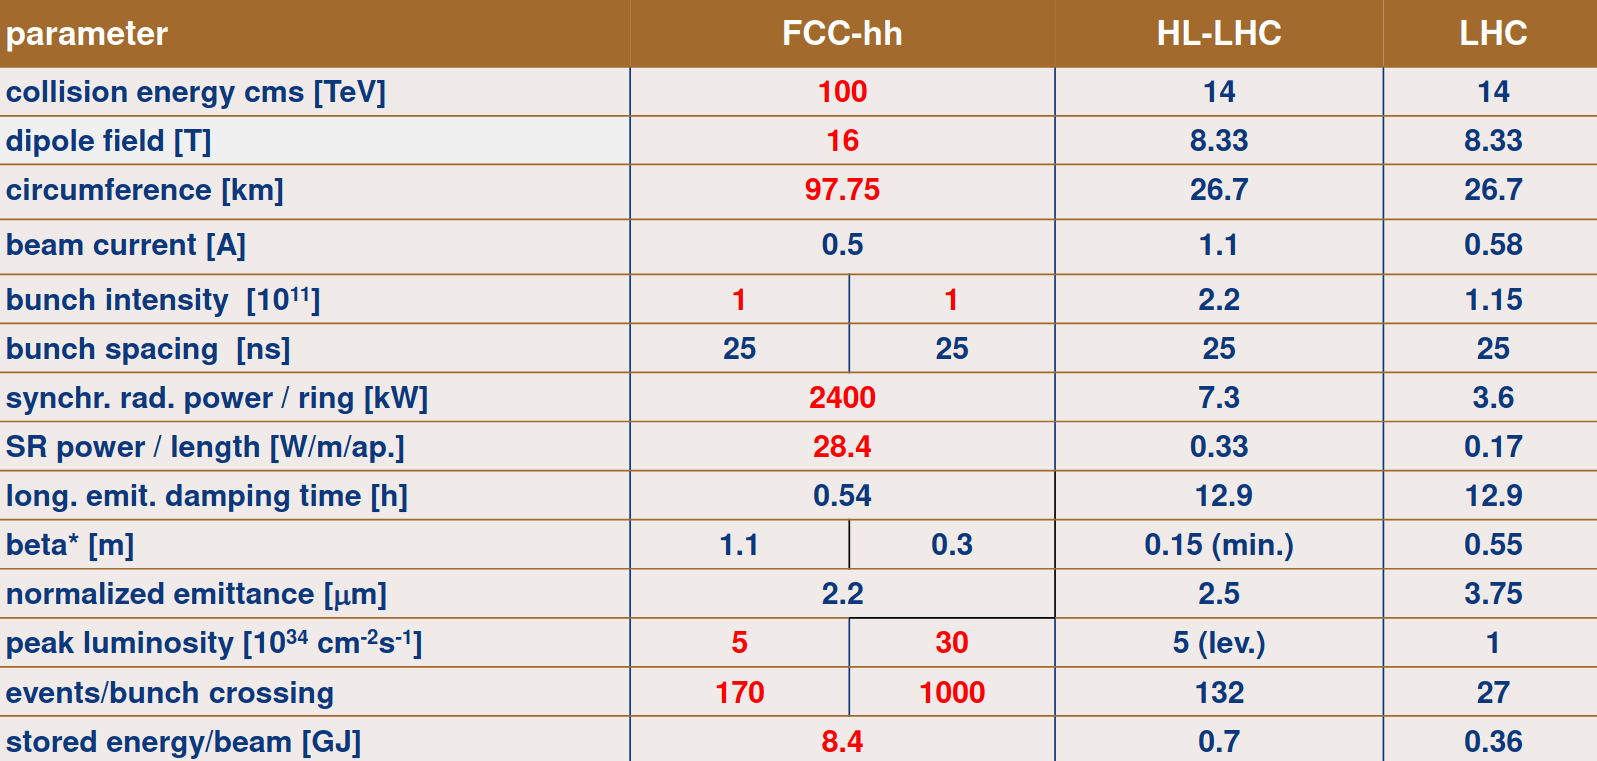
\includegraphics[width=1.0\linewidth]{figures/parameters-fcchh.png}\\
\end{frame}


%
% -----------------------------------------------------------------------------
%
\section{FCC Detectors}

\begin{frame}
  \frametitle{FCC-ee: CLD Detector}

  \begin{columns}[c]
    \column{.6\textwidth}
    \begin{center}
      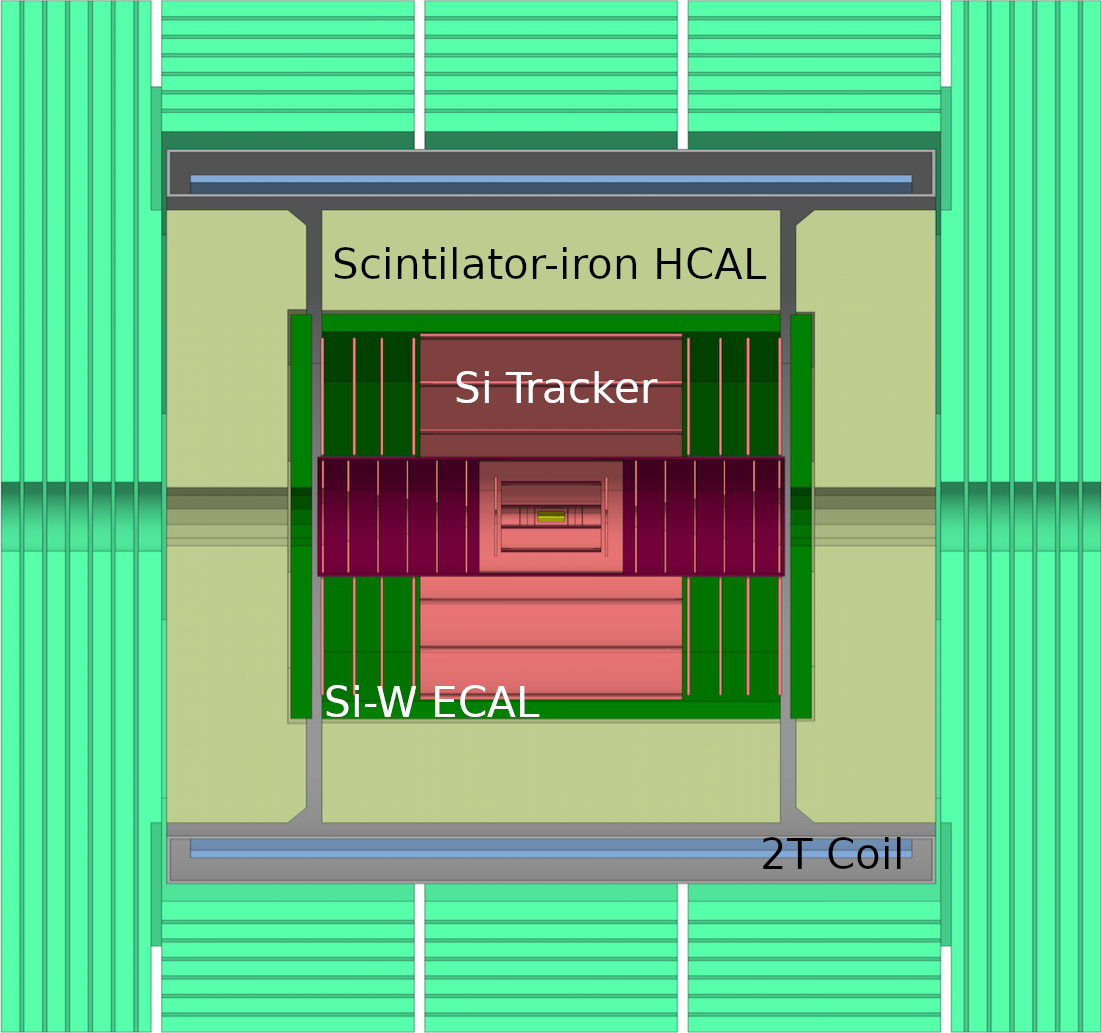
\includegraphics[width=0.9\linewidth]{figures/FCC_ee_CLD_text.png}
    \end{center}

    \column{.4\textwidth}
    \begin{itemize}
      \item Based on the detector for CLIC
      \item Silicon vertex detector and tracker
      \item 3D-imaging highly-granular calorimeter
      \item Coil outside calorimeter system
      \item Proved concept, understood performance
    \end{itemize}
  \end{columns}
\end{frame}

\begin{frame}
  \frametitle{FCC-ee: IDEA Detector}

  \begin{columns}[c]
    \column{.6\textwidth}
    \begin{center}
      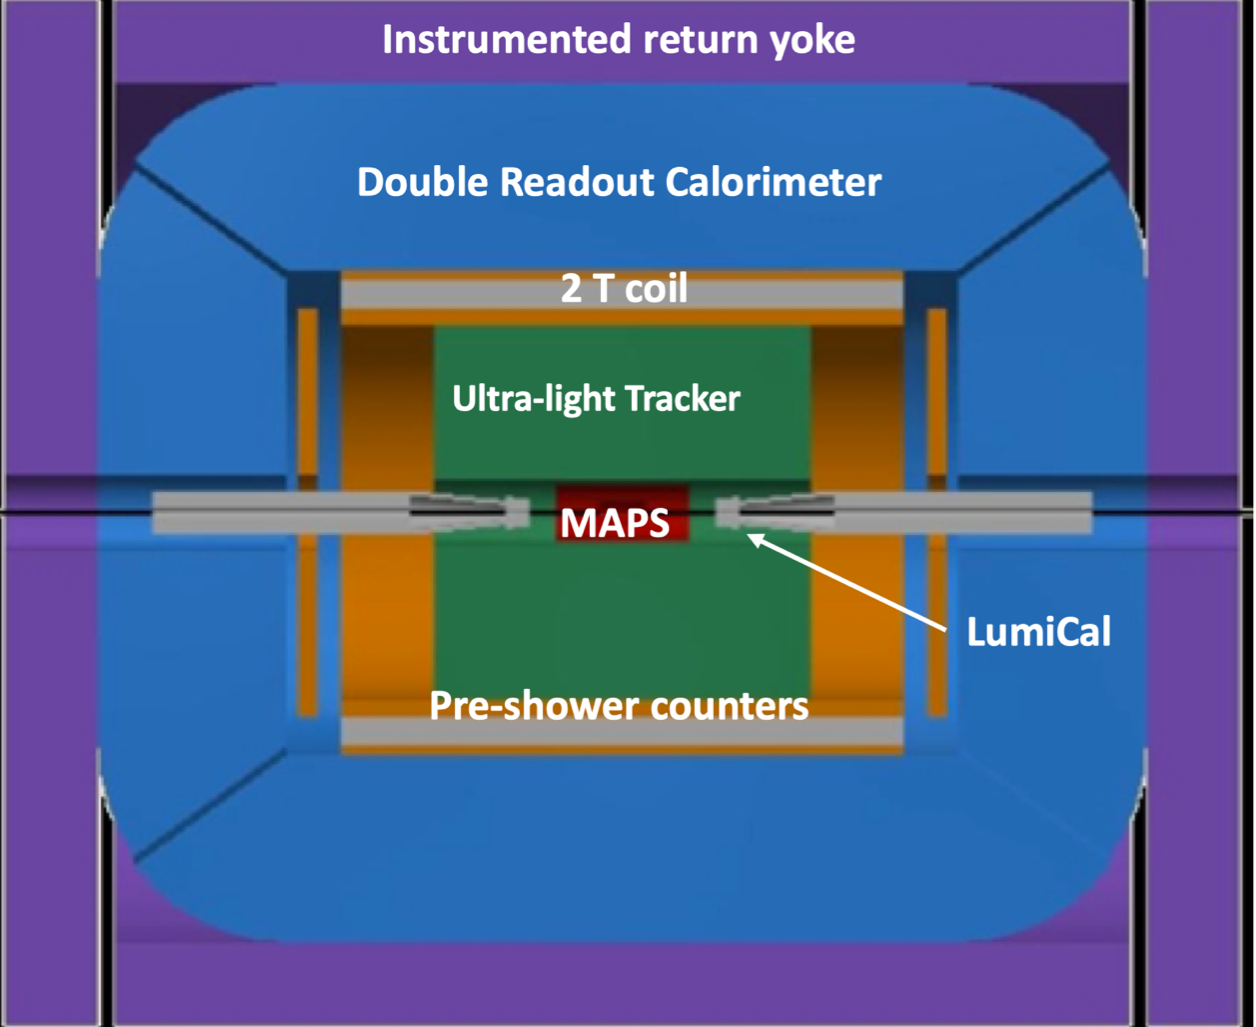
\includegraphics[width=\linewidth]{figures/FCC_ee_IDEA.png}
    \end{center}

    \column{.4\textwidth}
    \begin{itemize}
      \item New, innovative, possibly more cost-effective design
      \item Silicon vertex detector
      \item Short-drift, ultra-light wire chamber
      \item Dual-readout calorimeter
      \item Thin and light solenoid coil inside calorimeter system
    \end{itemize}
  \end{columns}
\end{frame}


%
% -----------------------------------------------------------------------------
%
\section{Calorimetry for FCC-ee}

\begin{frame}
  \frametitle{FCC-ee Calorimetry}

  \vspace{2ex}
  \begin{columns}[c]
    \column{.5\textwidth}
    \bluetext{Requirements:}
    \begin{itemize}
      \item Jet-jet inv.\ mass resolution to resolve $W$ from $Z$
            \begin{itemize}
              \item requires $\sim 3$\% ($\sim 30\% / \sqrt{E}$\,)
            \end{itemize}
      \item EM resolution at minimum 15\% to sustain jet resolution\\[-0.4ex]
            \begin{itemize}
              \item $B_\text{S} \rightarrow D_\text{S}K$ requires $\sim 5$\%
            \end{itemize}
      \item Crystal and LAr --- good EM resolution
      \item CALICE and Dual Readout --- good jet resolution
    \end{itemize}

    \column{.5\textwidth}
    \bluetext{Energy resolution param.:}
    \[ \frac{\sigma_\text{E}}{\langle E\,\rangle} = \frac{a}{\sqrt{E\,}} \oplus
                                                    \frac{b}{E} \oplus c \]

    \bluetext{Typical values:}
    \begin{center}
      \small
      \begin{tabular}{lcc}
        Technology   & $a$~[\%] & $c$~[\%] \\
        \midrule
        CALICE       & 15       & 1 \\
        Dual Readout & 10       & 1 \\
        LAr          & 9        & --- \\
        Crystal      & 3--5     & 0.5 \\
      \end{tabular}
    \end{center}
  \end{columns}

  \vspace{1ex}
  \redtext{High granularity and Particle Flow needed to achieve energy
           resolution of 3\%}
\end{frame}


\begin{frame}
  \frametitle{Noble Liquid Calorimetry for FCC-ee}

  \begin{columns}[c]
    \column{.5\textwidth}
    \bluetext{Key features:}
    \begin{itemize}
      \item Tested technology in ATLAS, D\O, H1, NA31/48/62
      \item Radiation hardness, long term stability
      \item Linear response, uniformity, high control over systematics
      \item Good energy and timing resolution
      \item Less than $10\%/\sqrt{E}$ demonstrated
    \end{itemize}

    \column{.5\textwidth}
    \begin{center}
      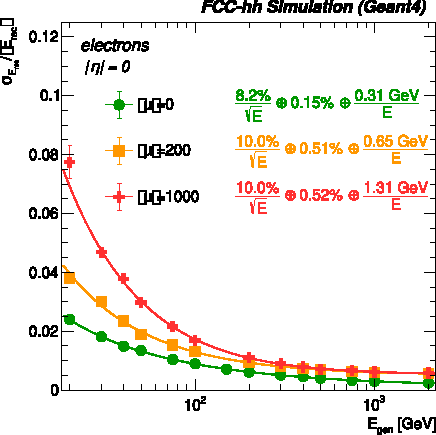
\includegraphics[width=.6\linewidth]{figures/FCC_hh_LAr_electron_performance_mu.pdf}
      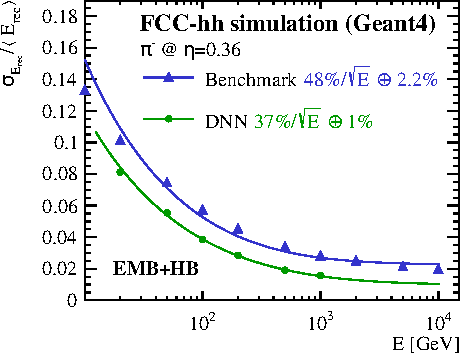
\includegraphics[width=.6\linewidth]{figures/FCC_hh_LAr_pion_performance.pdf}
    \end{center}
  \end{columns}
\end{frame}


\begin{frame}
  \frametitle{CALICE}

  Collaboration of mostly Si/Tungsten based high granularity calorimeters\\[1ex]
  \bluetext{Traits:}
  \begin{columns}[c]
    \column{.4\textwidth}
    \begin{itemize}
      \item Large area silicon detectors
      \item Si Photomultipliers
      \item Highly integrated front-end electronics with timing
      \item Very large number of channels
    \end{itemize}

    \column{.6\textwidth}
    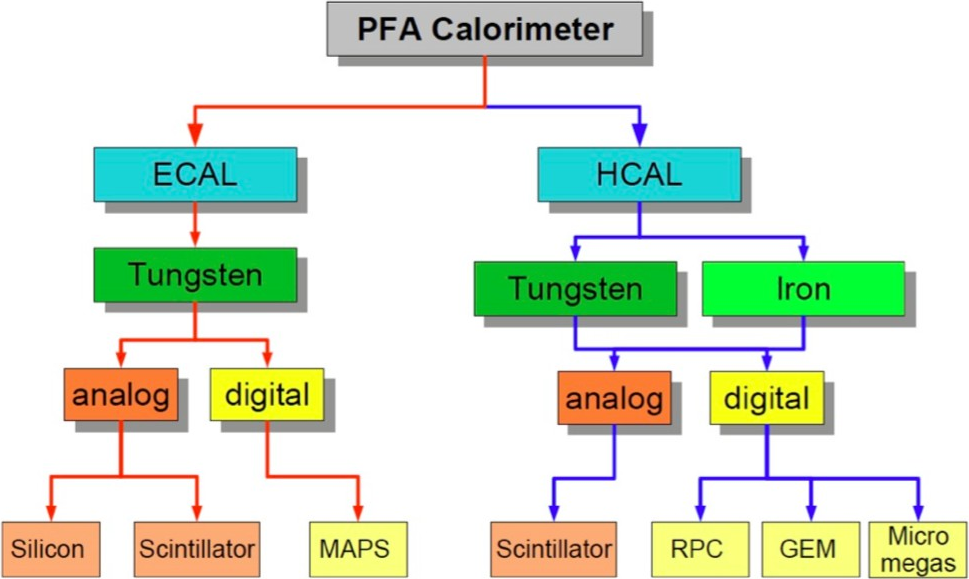
\includegraphics[width=\linewidth]{figures/CALICE_diagram.png}
  \end{columns}
\end{frame}


\begin{frame}
  \frametitle{FCC-ee: CLD Calorimeter}

  \bluetext{CLD proposal:}
  \begin{itemize}
    \item 40 layers SiW ECAL (22 $X_0$)
    \item 60 layers Scint/Steel HCAL (7.5 $\lambda_\text{I}$ +
          1 $\lambda_\text{I}$ in ECAL)
  \end{itemize}

  \begin{center}
    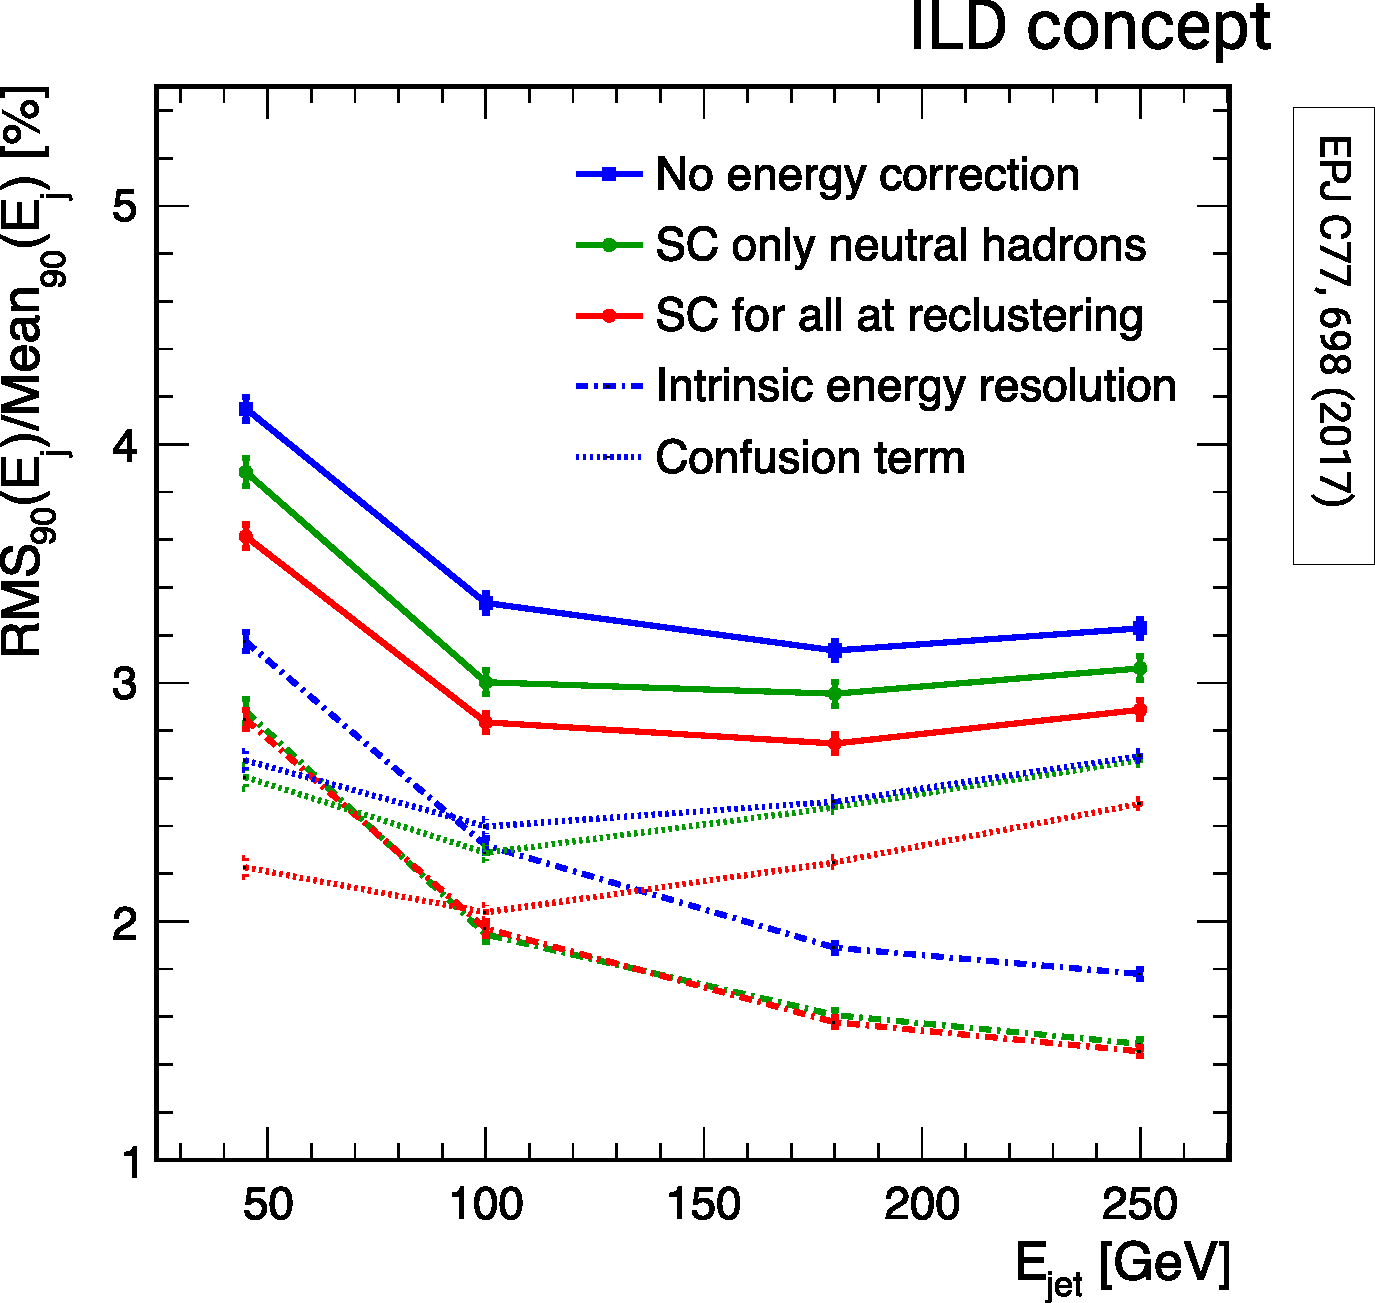
\includegraphics[width=0.41\linewidth]{figures/CLD_jet_performance.pdf}
    \hspace{7mm}
    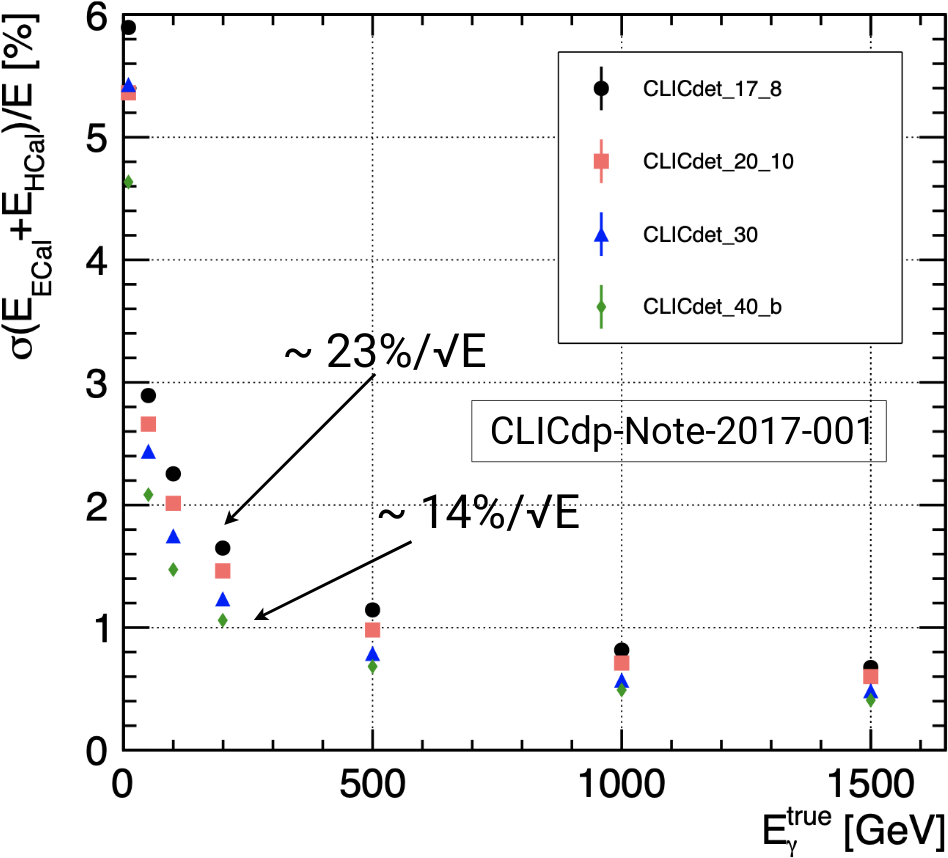
\includegraphics[width=0.41\linewidth]{figures/CLD_photon_performance.png}
  \end{center}
\end{frame}


\begin{frame}
  \frametitle{FCC-ee: IDEA Calorimeter}

  \bluetext{Traits:}
  \begin{itemize}
    \item Dual readout calorimeter with 1.5~mm pitch between
          Cherenkov and Scintillation fibers
    \item Single EM + HAD sampling calorimeter
    \item No mechanical longitudinal segmentation ($\sim 7 \lambda_\text{I}$)
    \item Good EM intrinsic energy resolution
    \item Excellent hadronic resolution
  \end{itemize}

  \vspace*{-2.1ex}
  \begin{center}
    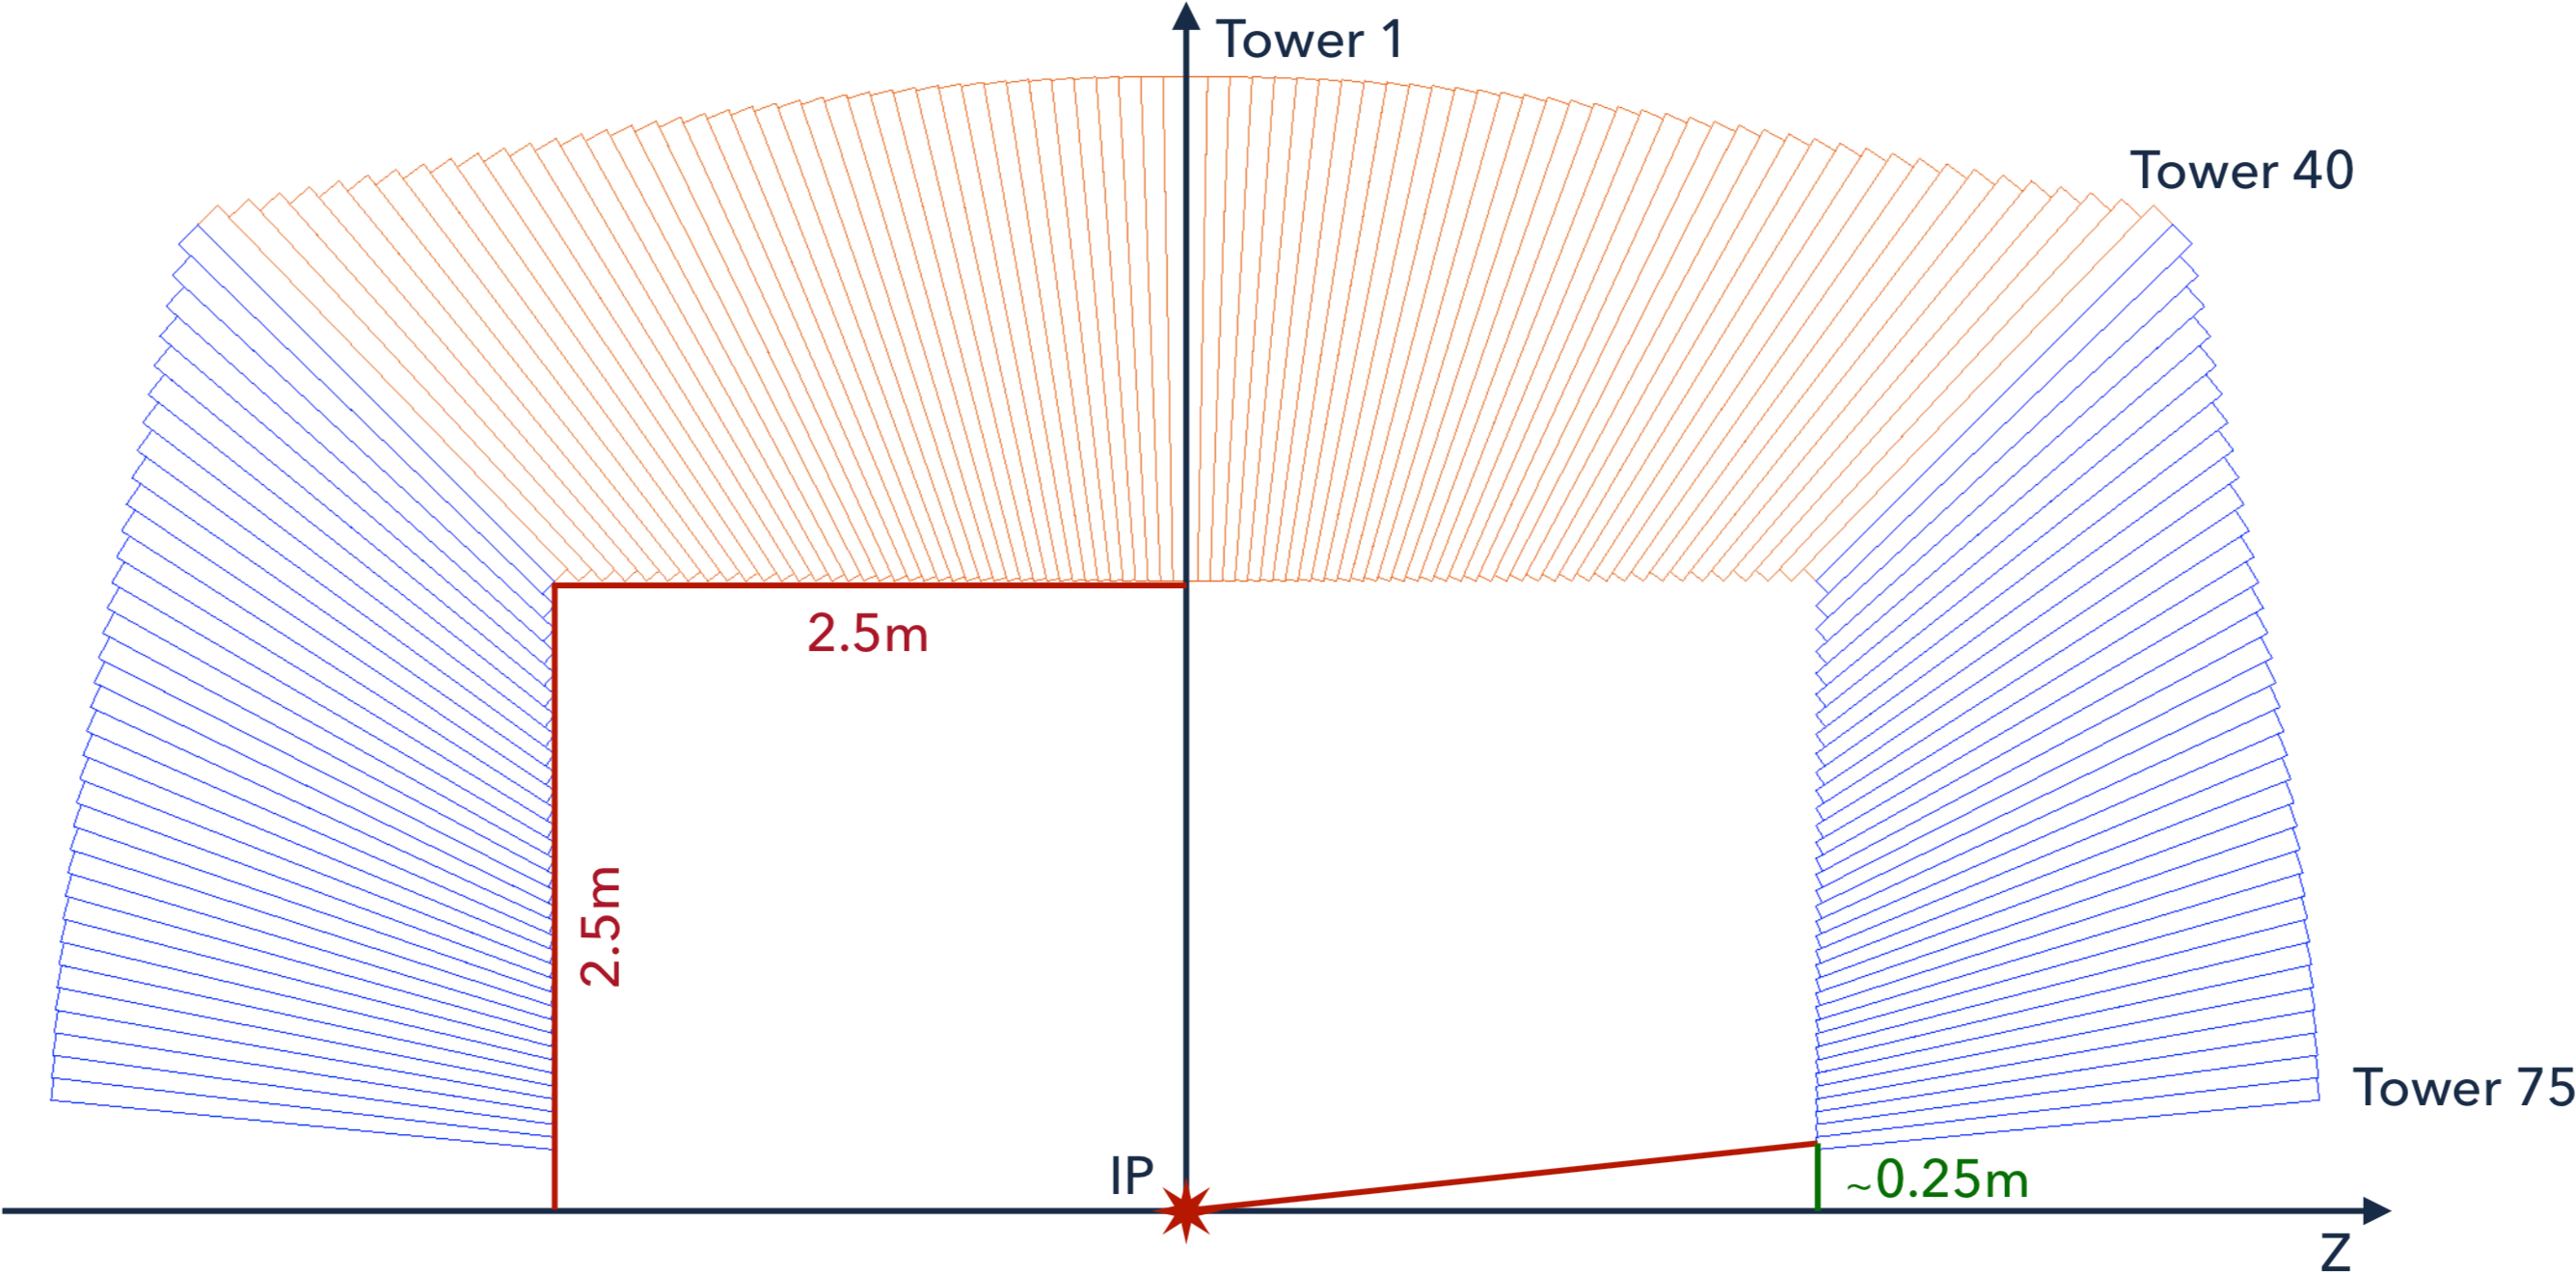
\includegraphics[width=.52\linewidth]{figures/IDEA_calorimeter_flatview.png}
  \end{center}
\end{frame}


\begin{frame}
  \frametitle{Dual Readout Calorimeter}

  \begin{columns}[c]
    \column{.5\textwidth}
    \bluetext{Principle:}
    \begin{itemize}
      \item Correct $f_\text{em}$ in every event
            \begin{itemize}
              \item Main source of fluctuations
            \end{itemize}
      \item Fibers pointing toward IP
            \begin{itemize}
              \item \bluetext{Scintillating:} sense charged
              \item \bluetext{Clear:} sense Cherenkov, mostly electrons
            \end{itemize}
    \end{itemize}

    \column{.5\textwidth}
    \begin{center}
      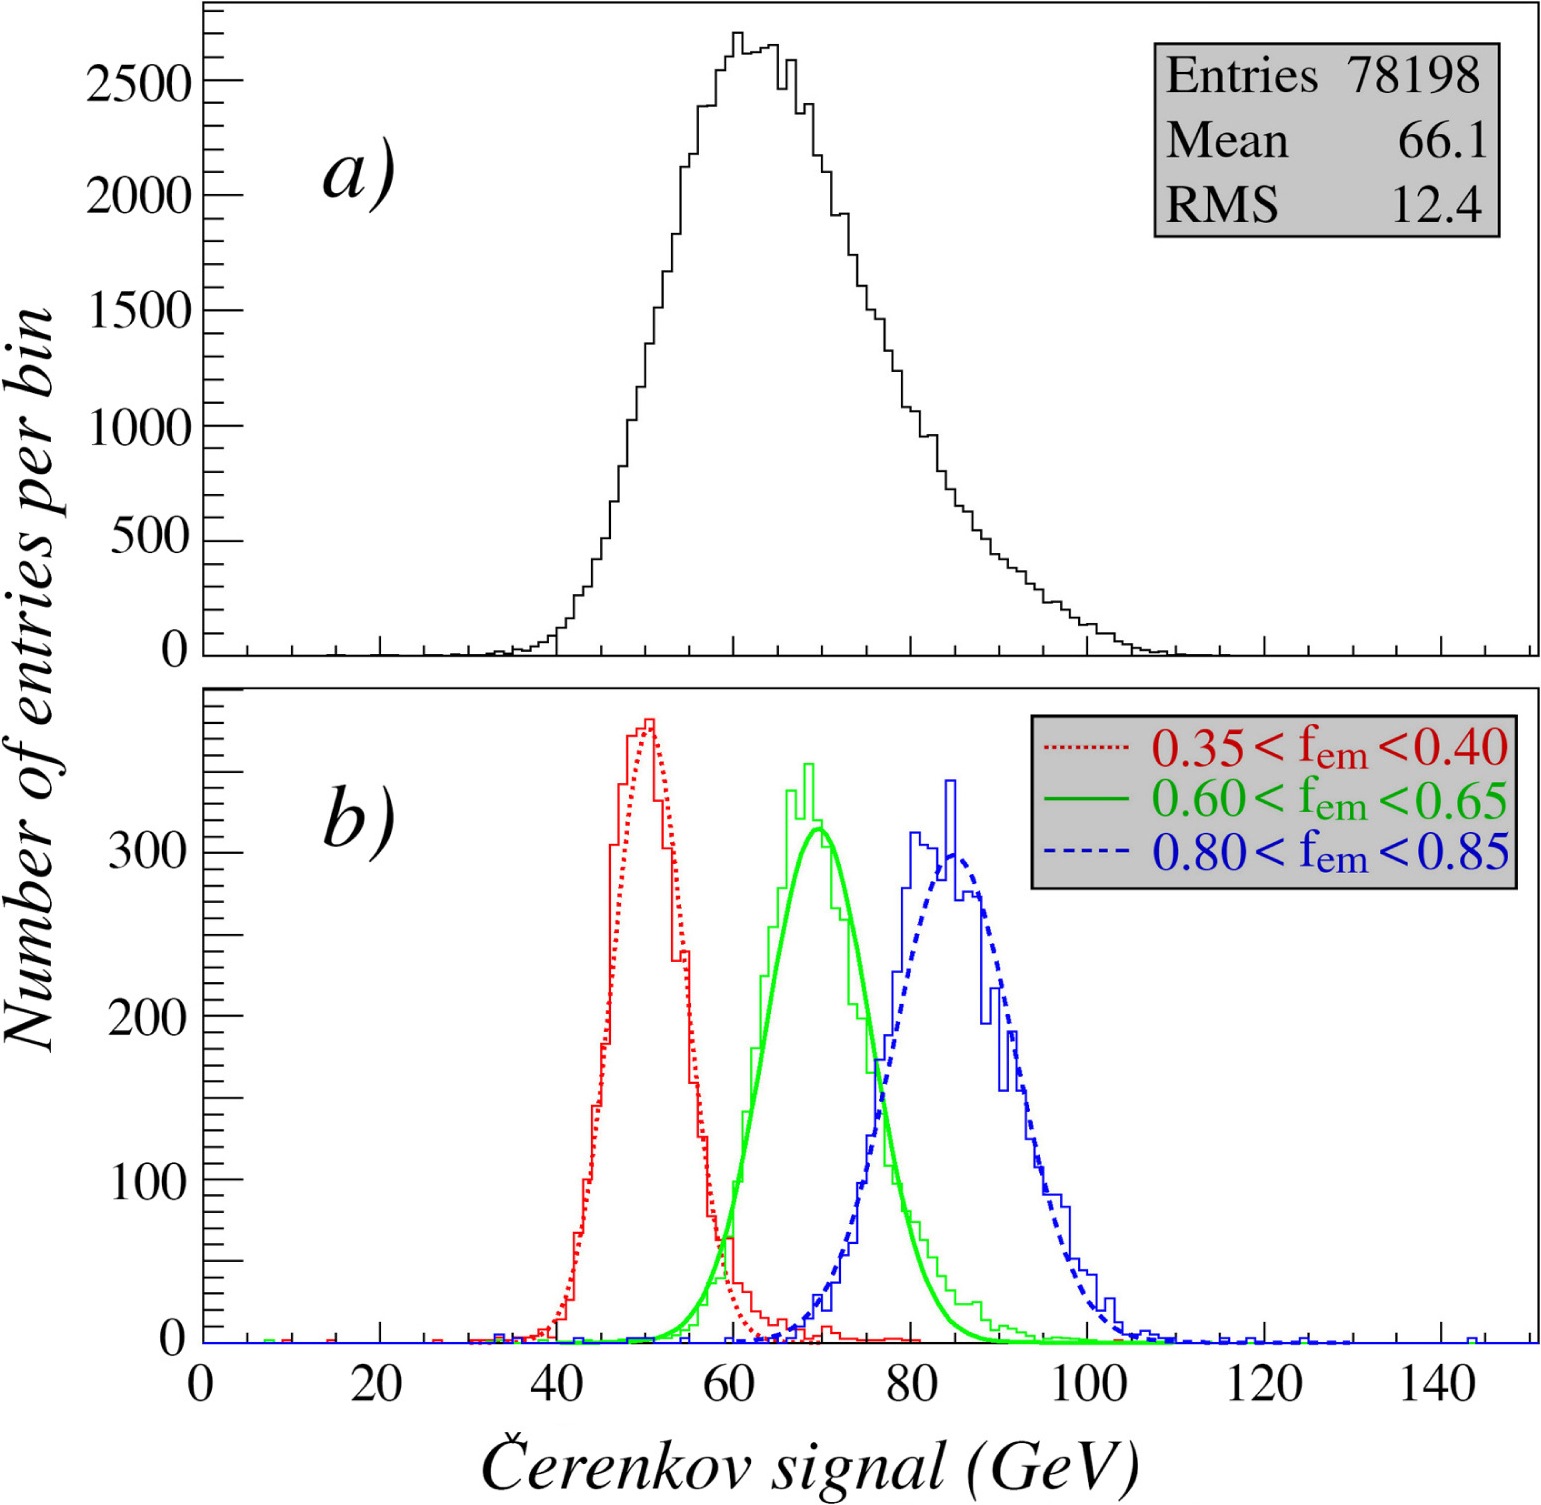
\includegraphics[width=.8\linewidth]{figures/dual_readout_signal_example.png}
      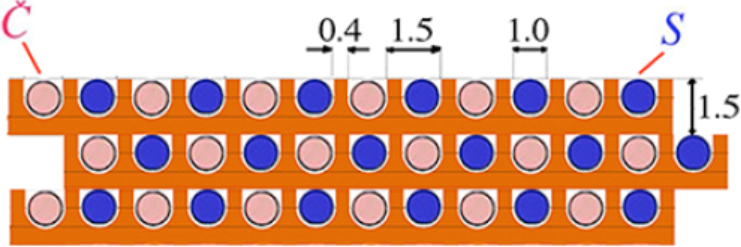
\includegraphics[width=.8\linewidth]{figures/IDEA_calorimeter_fibers.png}
    \end{center}
  \end{columns}
\end{frame}


\begin{frame}
  \frametitle{Crystal Calorimeters}

  \begin{columns}[c]
    \column{.5\textwidth}
    \bluetext{Traits:}
    \begin{itemize}
      \item Mostly investigated for CEPC
      \item Used by CMS
      \item Homogeneous structure
      \item Has optimal intrinsic energy resolution:
            $\sim 3\%/\sqrt{E\,} \, \oplus \sim 1\%$
    \end{itemize}

    \column{.5\textwidth}
    \begin{center}
      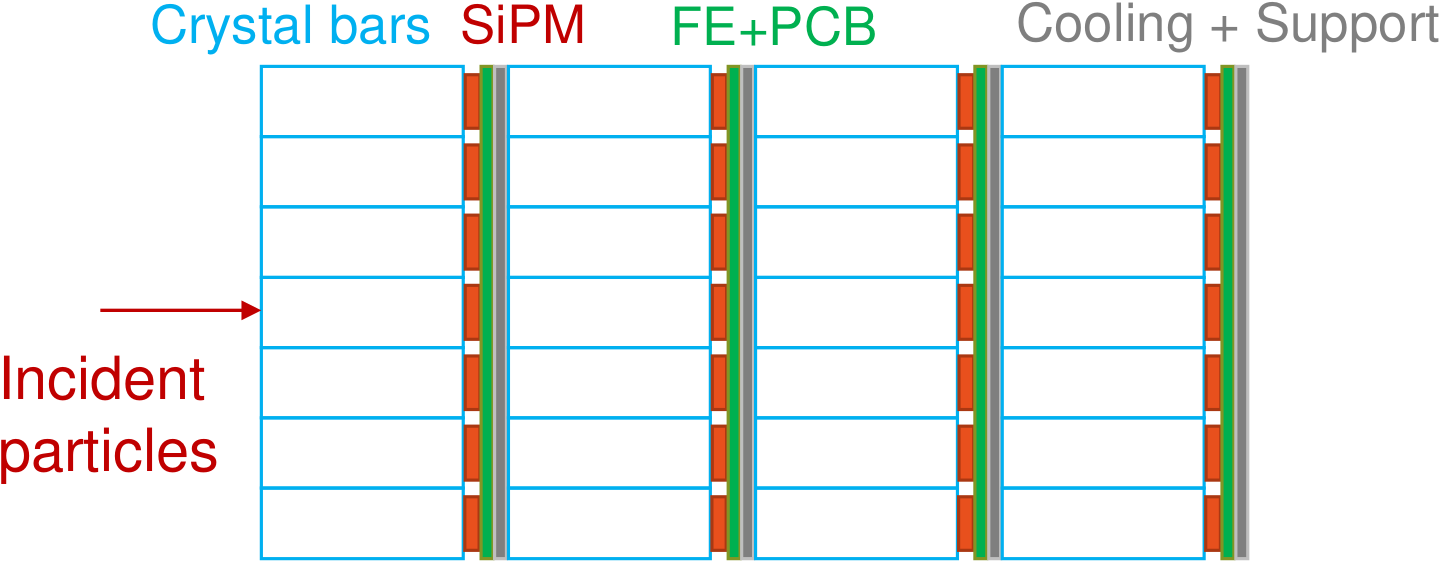
\includegraphics[width=\linewidth]{figures/CEPC_crystal_calo_design1.png}%
      \vspace{2ex}
      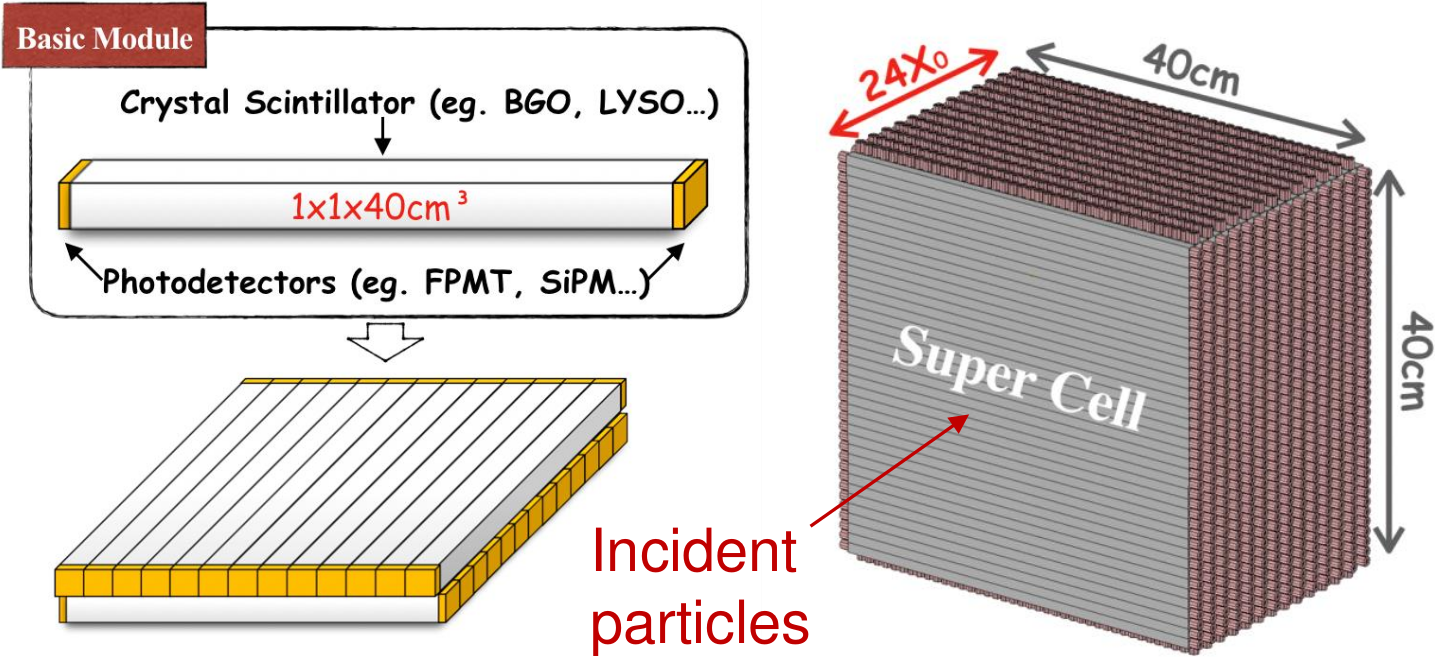
\includegraphics[width=\linewidth]{figures/CEPC_crystal_calo_design2.png}
    \end{center}
  \end{columns}
\end{frame}


%
% -----------------------------------------------------------------------------
%
\section{Improvements in Noble-liquid for FCC-ee}

\begin{frame}
  \frametitle{Improvements in Noble Liquid Calorimetry}

  \begin{itemize}
    \item Noble liquid is viable technology for FCC-ee detectors
    \item New round of optimizations started with multiple R\&D projects
    \item Both hardware and software improvements are required to get to 3\%
    \item Design driven by Particle Flow
  \end{itemize}

  \vspace{-1.5em}
  \begin{center}
    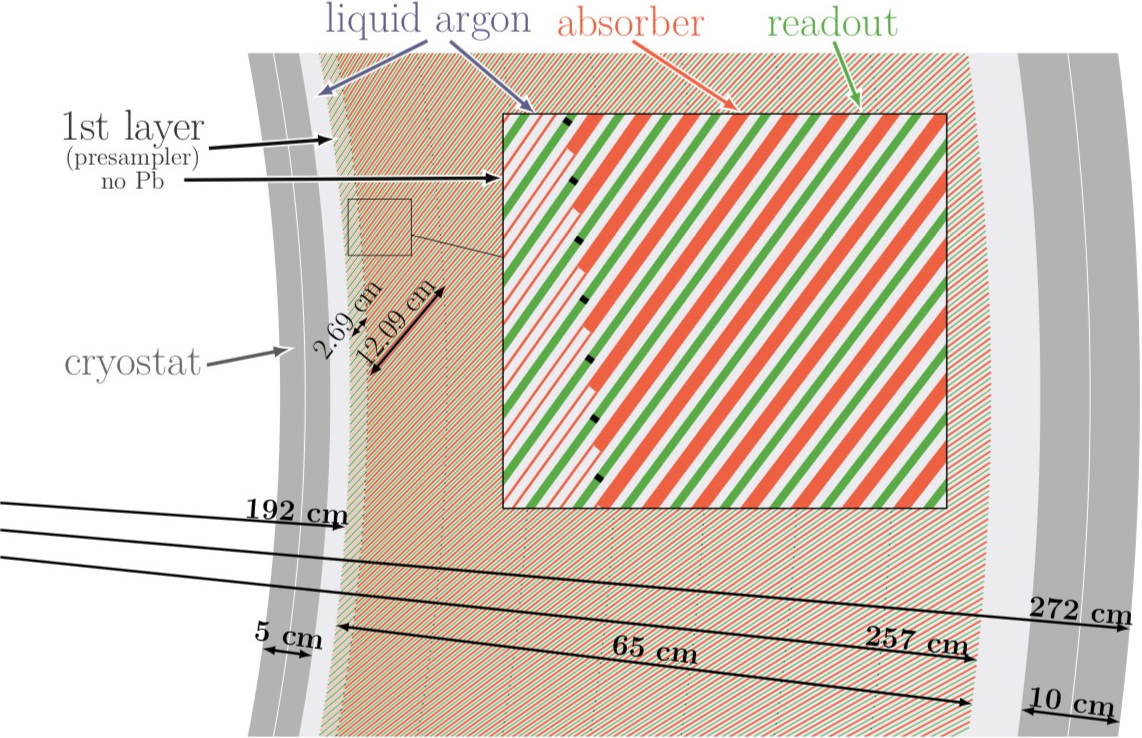
\includegraphics[align=c,width=0.47\linewidth]{figures/FCC_hh_LAr_diagram.png}%
    \hfill
    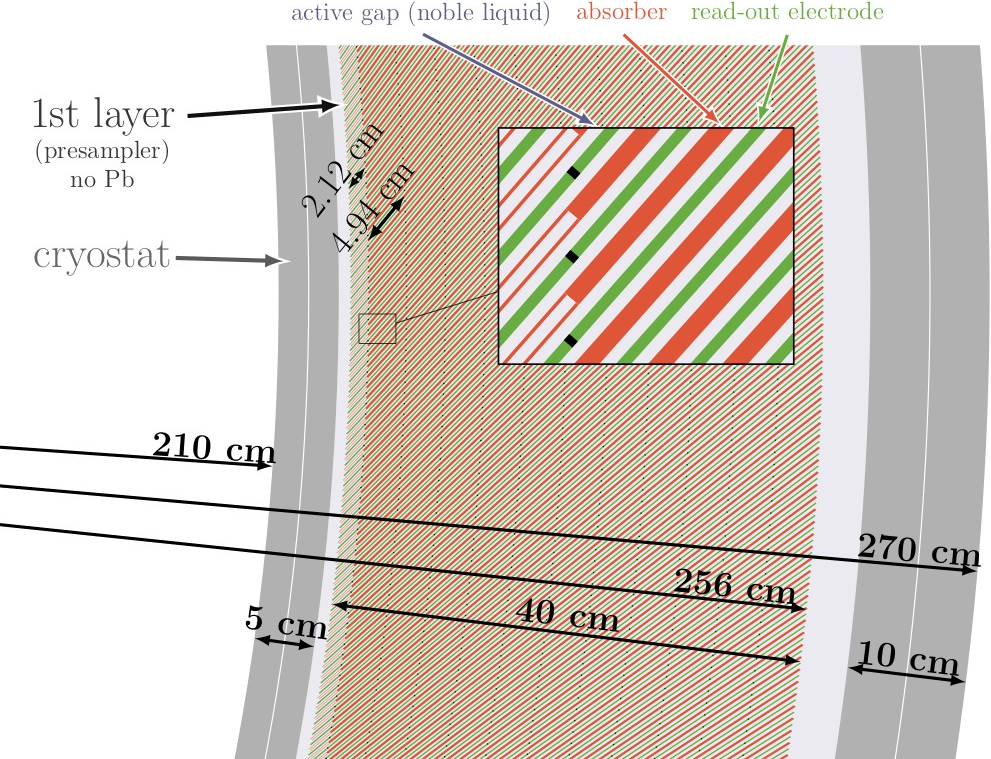
\includegraphics[align=c,width=0.47\linewidth]{figures/FCC_ee_LAr_diagram.png}\\[.5em]
    FCC-hh \hspace{16em} FCC-ee
  \end{center}
\end{frame}


\begin{frame}
  \frametitle{Particle Flow}

  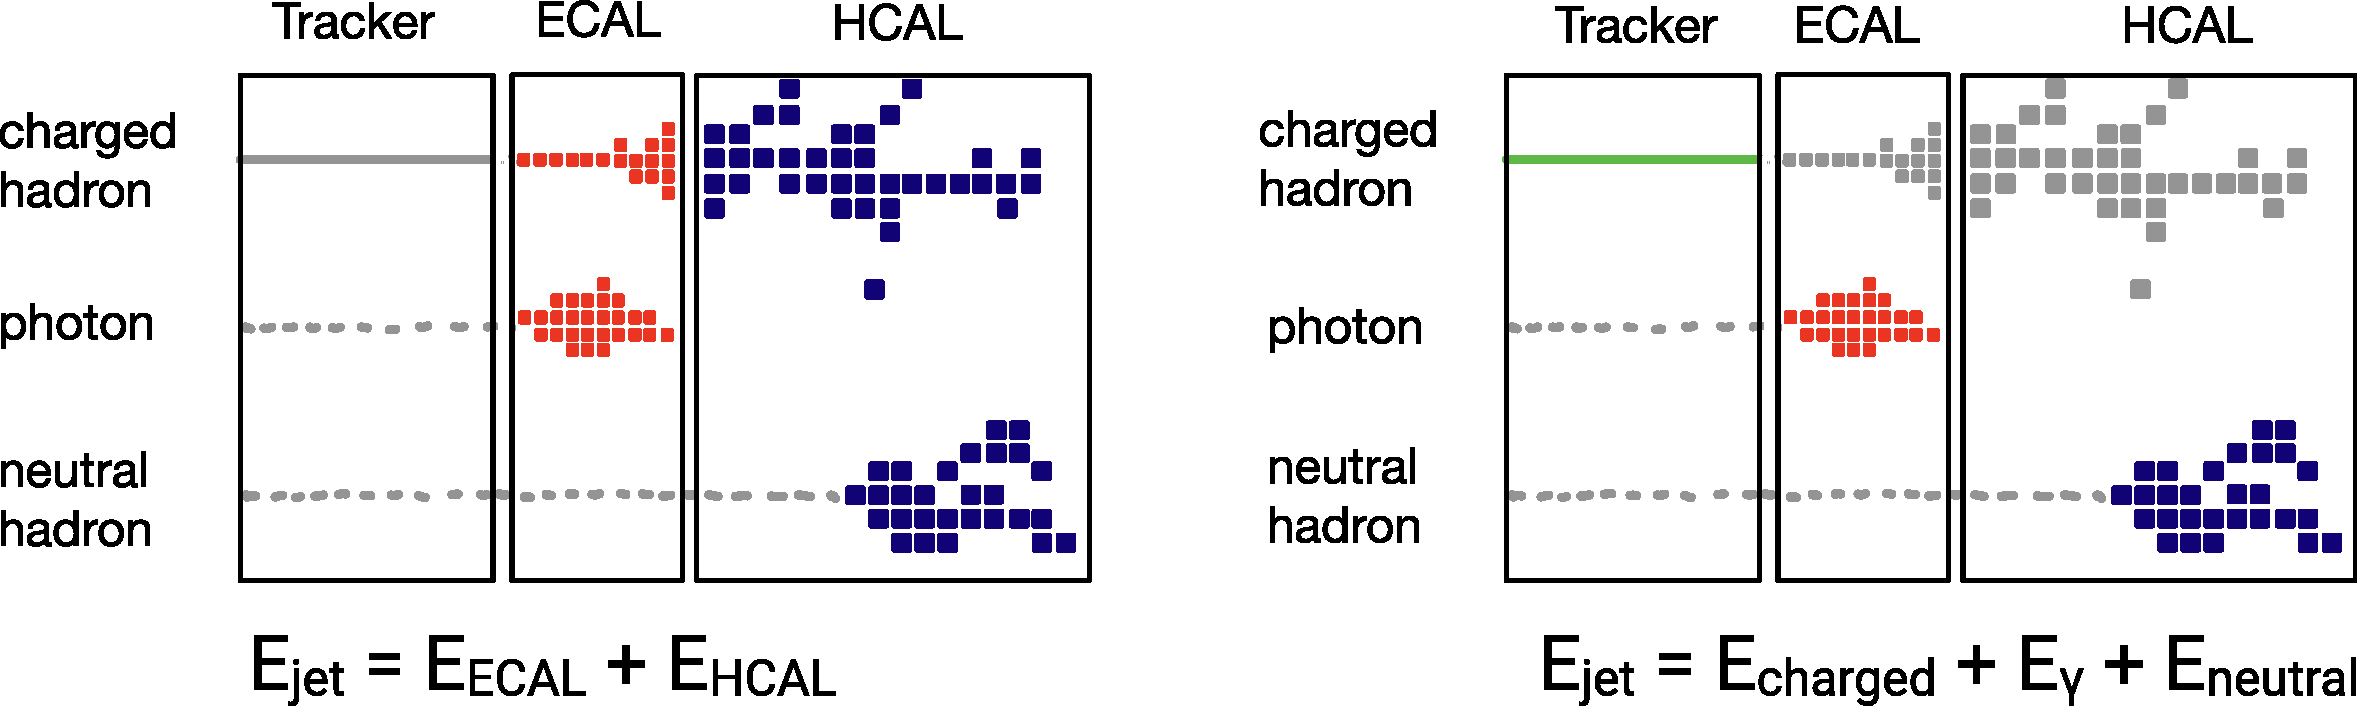
\includegraphics[width=\linewidth]{figures/particle_flow_diagram.pdf}
  \vspace{-1.5ex}
  \hspace{6.7em} 30\% + 70\% \hspace{14.5em} 60\% + 30\% + 10\%

  \vspace{-1ex}
  \bluetext{Idea:}
  \begin{columns}[c]
    \column{.5\textwidth}
    \begin{itemize}
      \item Reconstruct every particle in the event with the best possible
            precision
      \item Combine the measurements in subdetectors in an optimal way
    \end{itemize}

    \column{.5\textwidth}
    \begin{itemize}
      \item Charged particles dominated by tracker
      \item Calorimetry mostly for neutral particles
      \item \bluetext{Enemy: Confusion}
    \end{itemize}
  \end{columns}

\end{frame}

\begin{frame}
  \frametitle{Hardware Improvements FCC-ee I}

  \begin{columns}[c]
    \column{.5\textwidth}

    \bluetext{Higher granularity:}
    \begin{itemize}
      \item Both transverse and in depth
      \item Factor of 10x in comparison to ATLAS LAr (220k $\rightarrow$ ~2M
            cells)
      \item Using simpler design --- PCBs
      \item Signal traces are embedded in PCB
      \item More signal traces $\rightarrow$ more noise
      \item High longitudinal segmentation mitigates gap widening towards high
            radius
      \item More signal traces $\rightarrow$ high density feedthroughs
    \end{itemize}

    \column{.5\textwidth}

    \begin{center}
      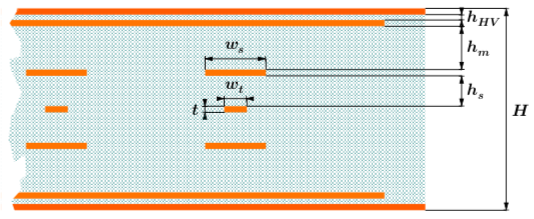
\includegraphics[width=\linewidth]{figures/fcc-lar-electrodes.png}\\[1em]
      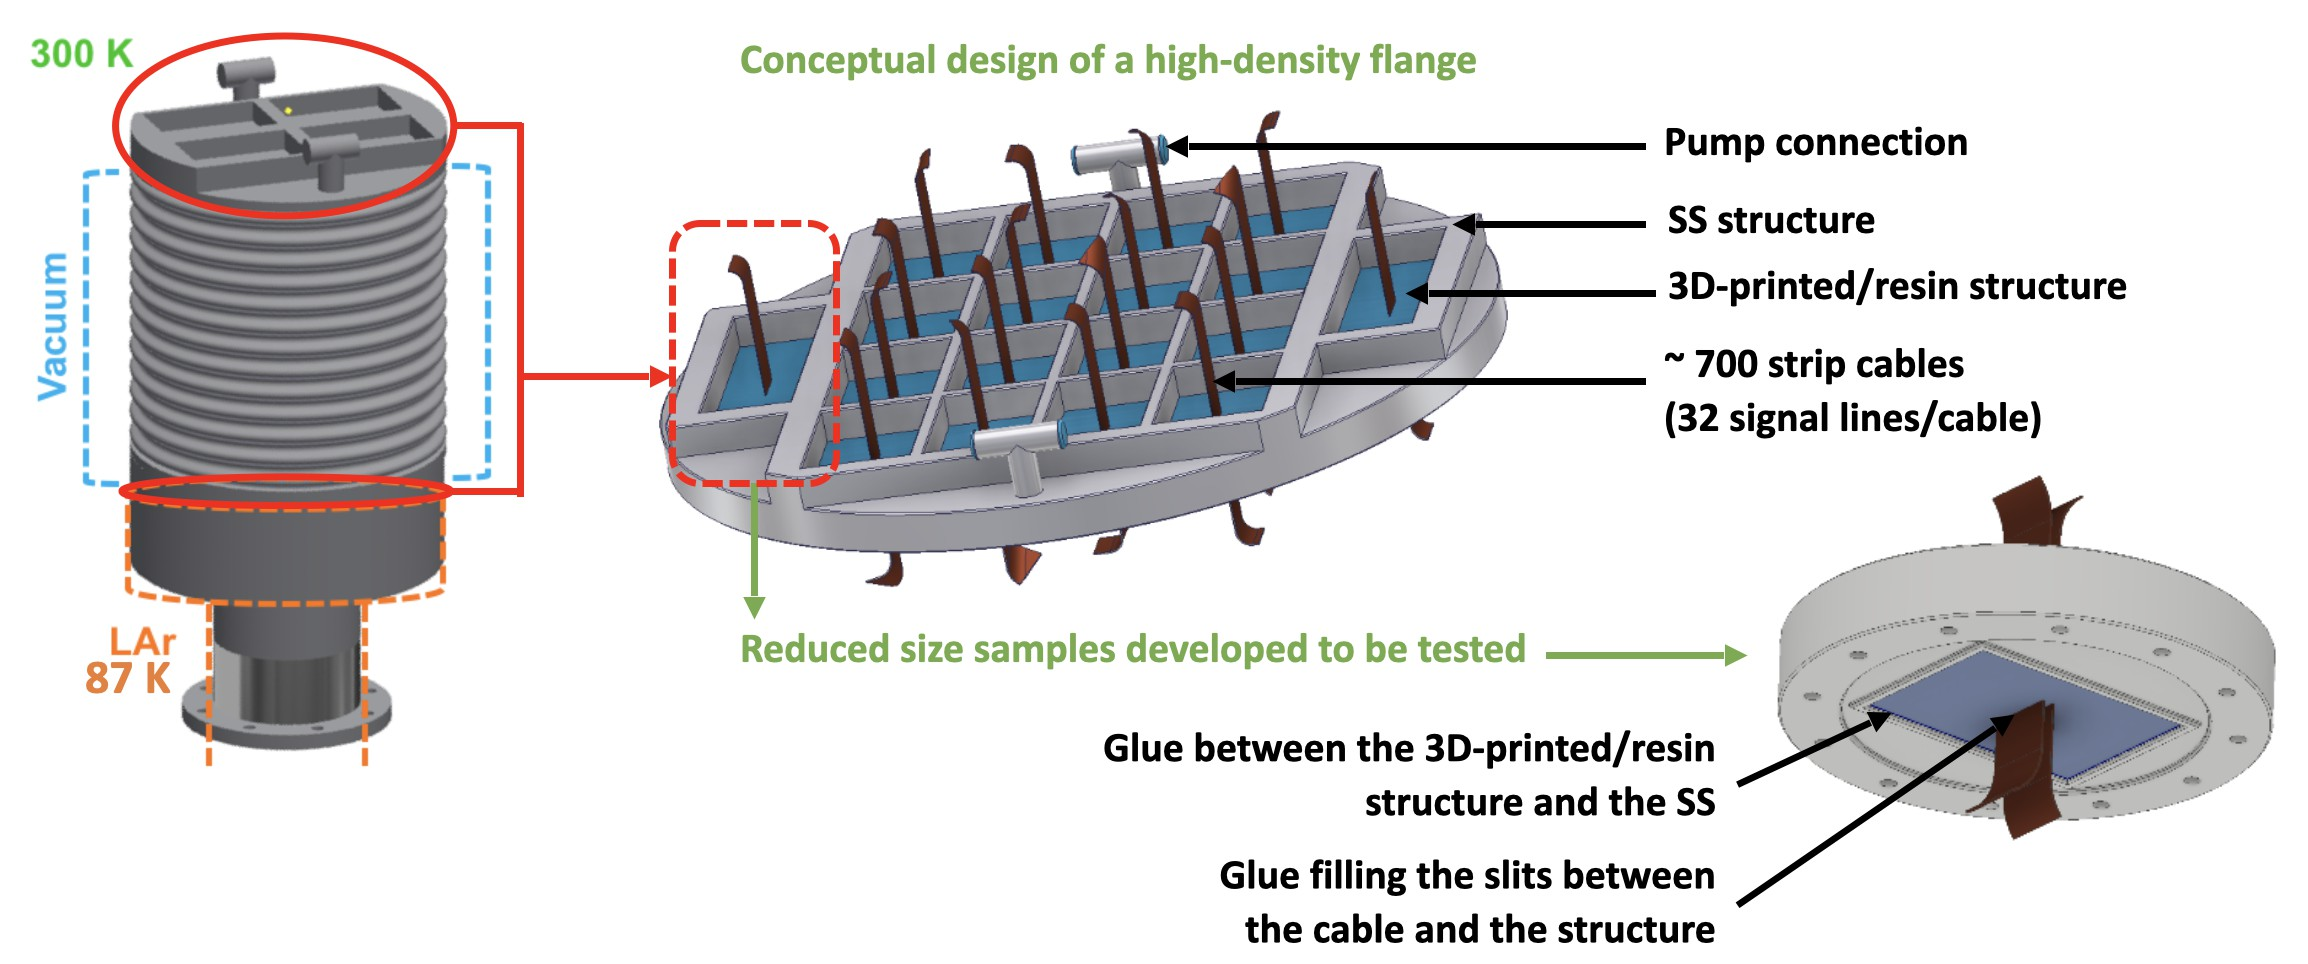
\includegraphics[width=\linewidth]{figures/fcc-lar-feedthroughs.png}
    \end{center}
  \end{columns}
\end{frame}


\begin{frame}
  \frametitle{Hardware Improvements for FCC-ee II}

  \begin{columns}[c]
    \column{.5\textwidth}

    \bluetext{Cryostat vessel:}
    \begin{itemize}
      \item Important for low energy particle measurements (bellow 300 MeV)
      \item Carbon fiber reinforced cryostat under investigation
      \item Vacuum vessel shared between solenoid and calorimeter
    \end{itemize}
    \bluetext{Electronics:}
    \begin{itemize}
      \item Warm or Cold electronics
      \item Charge or current pre-amplifiers
      \item Dynamic range: 14--16 bits
      \item Time resolution optimization
    \end{itemize}

    \column{.5\textwidth}

    \begin{center}
      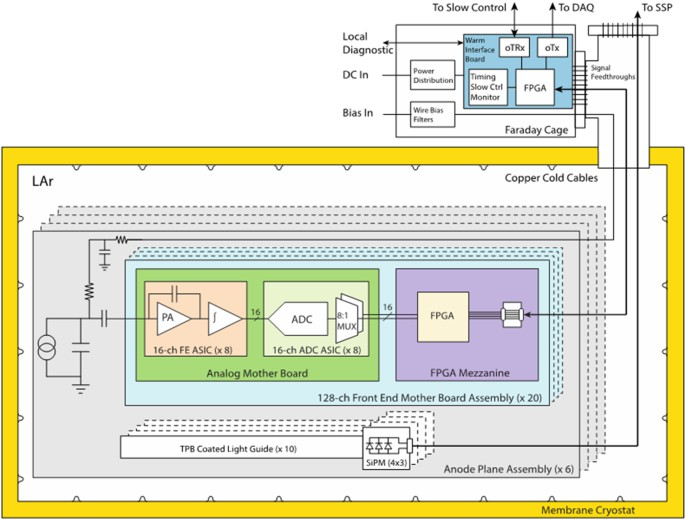
\includegraphics[width=0.7\linewidth]{figures/protodune-electronics.png}\\[0.5em]
      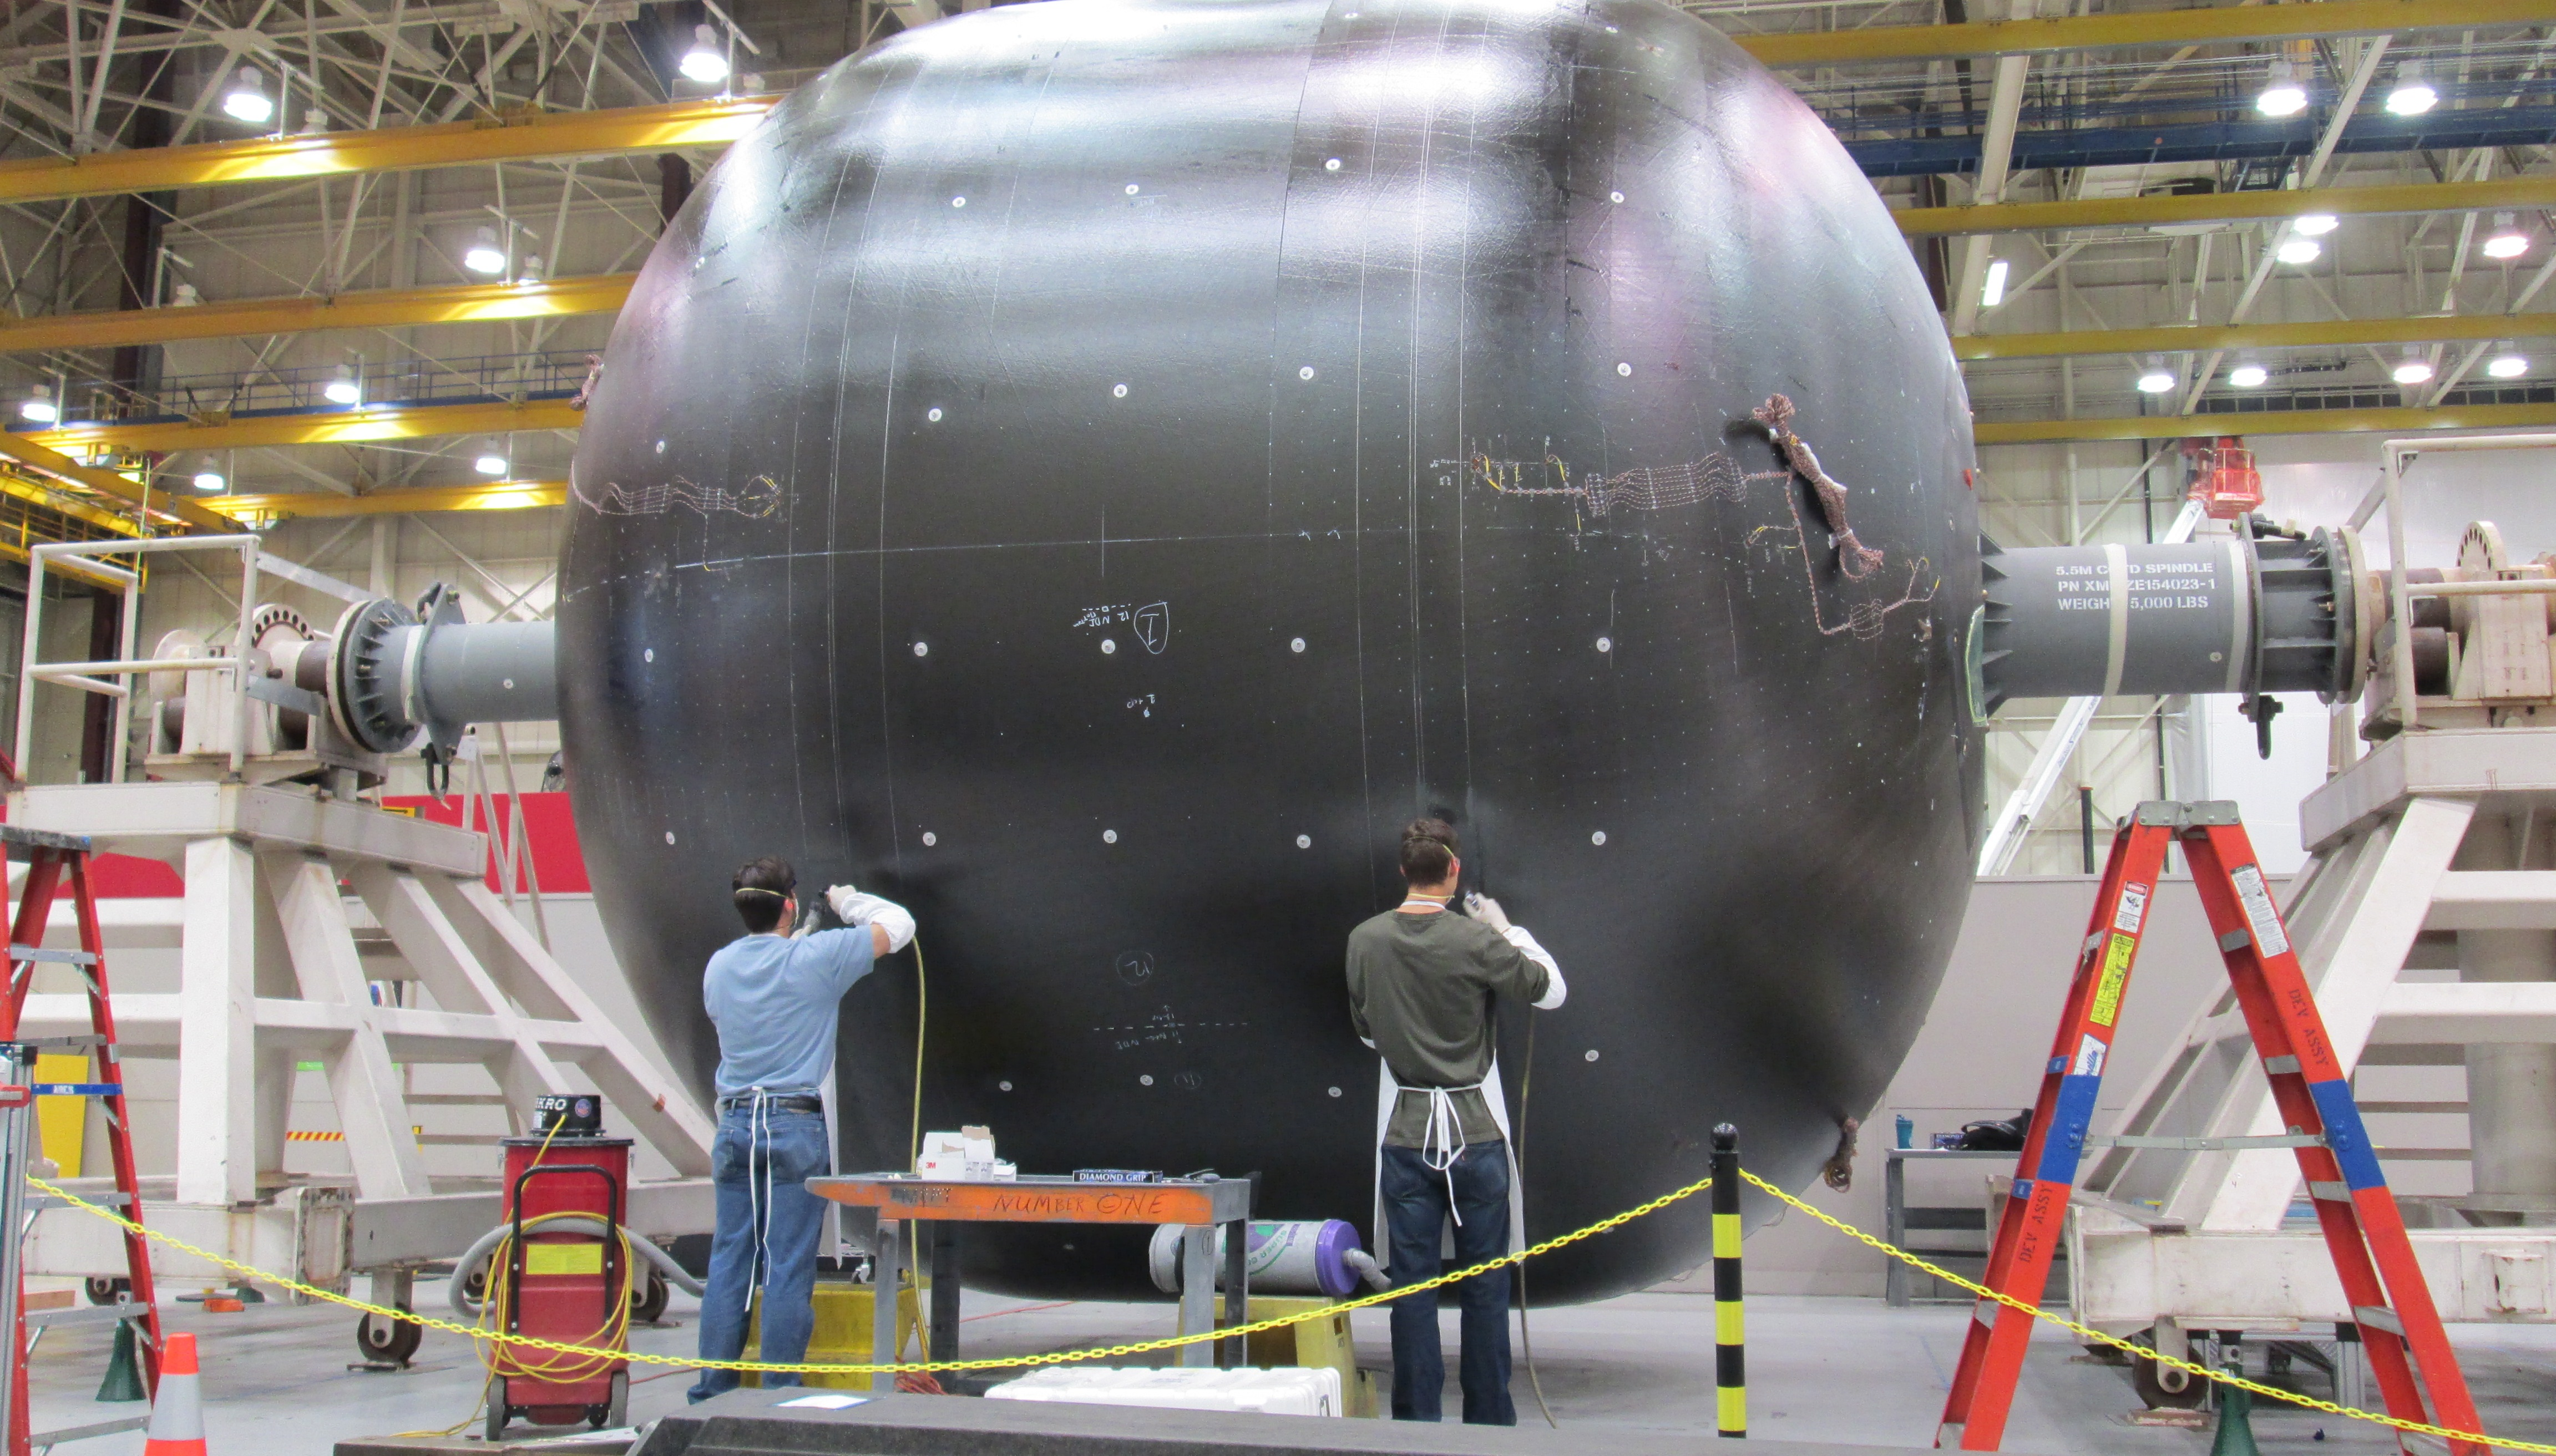
\includegraphics[width=0.9\linewidth]{figures/nasa-cryotank.jpg}
    \end{center}
  \end{columns}
\end{frame}


\begin{frame}
  \frametitle{Hardware Improvements for FCC-ee III}

  \begin{columns}[c]
    \column{.5\textwidth}

    \bluetext{Material \& Construction}
    \begin{itemize}
      \item Alignment and uniformity affects constant term
      \item Active material (Krypton, \dots)
      \item Absorber material (Tungsten, \dots)
      \item Absorber and sensitive gap thickness
      \item Plate inclination, layer depths, cell merging
      \item Interplay between sub-systems
    \end{itemize}

    \column{.5\textwidth}

    \begin{center}
      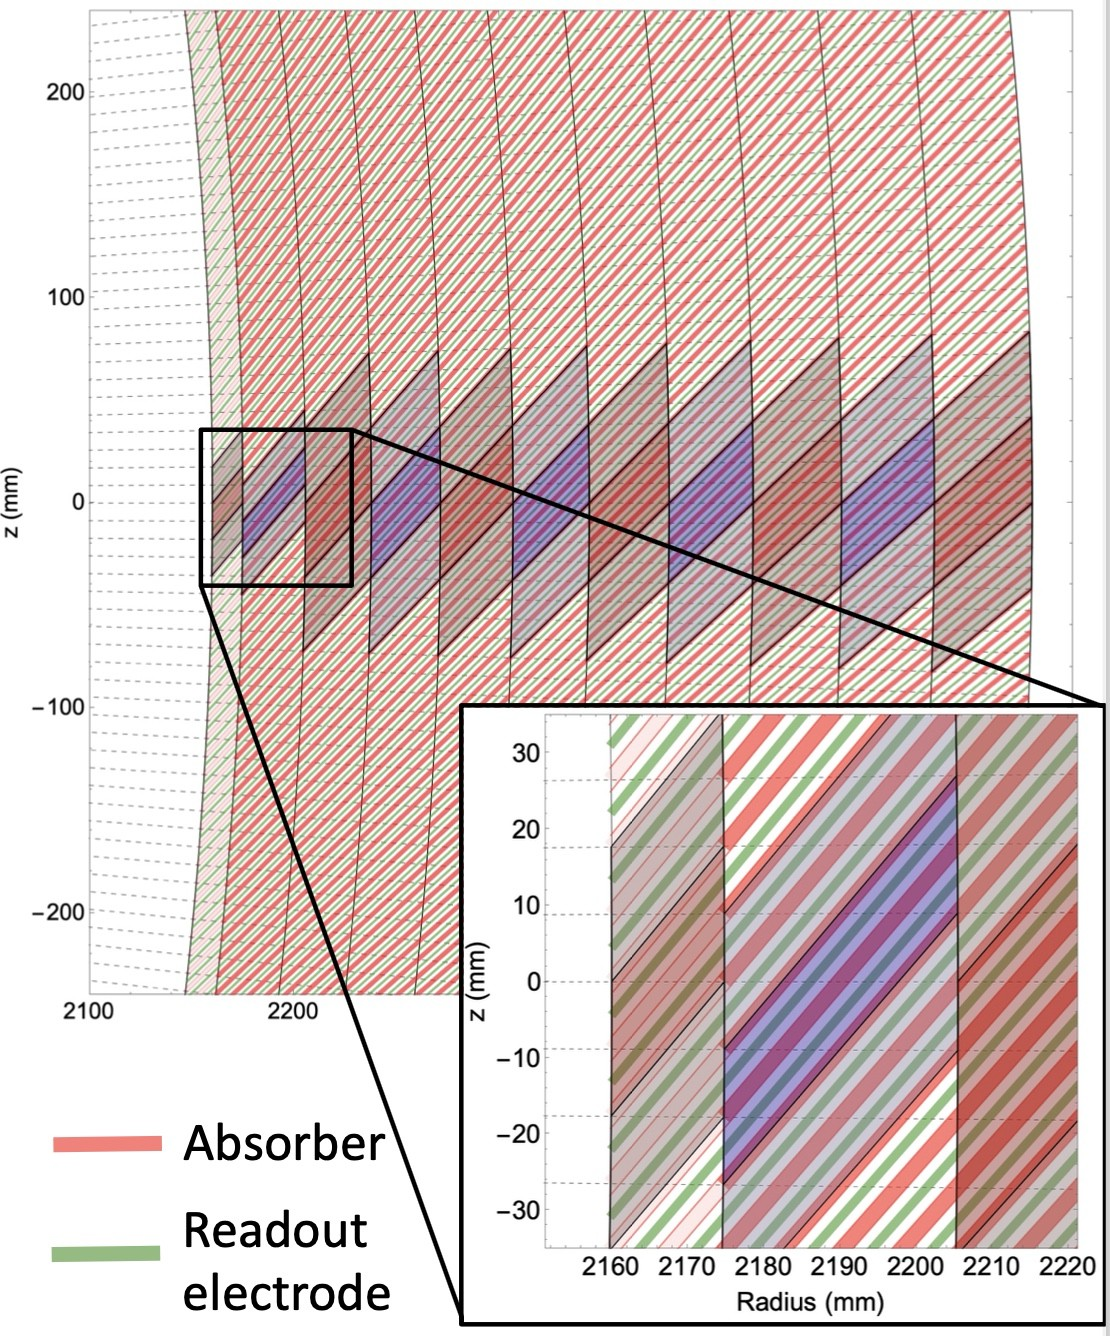
\includegraphics[width=0.7\linewidth]{figures/fcc-lar-segmentation.png}
    \end{center}
  \end{columns}
\end{frame}

\begin{frame}
  \frametitle{Software Improvements for FCC-ee}

  \begin{columns}[c]
    \column{.6\textwidth}
    \begin{itemize}
      \item New generic framework Key4HEP emerges from the FCCSW and iLCSoft
      \item Based on Gaudí but uses Podio
      \item Integrates tools from simulation, detector description to
            reconstruction
      \item Integration of Particle Flow algorithm (Pandora SDK)
      \item Reimplementation of clustering algorithm (CLUE)
      \item Replacement of ECal in CLD or IDEA by LAr calorimeter
    \end{itemize}

    \column{.4\textwidth}
    \begin{center}
      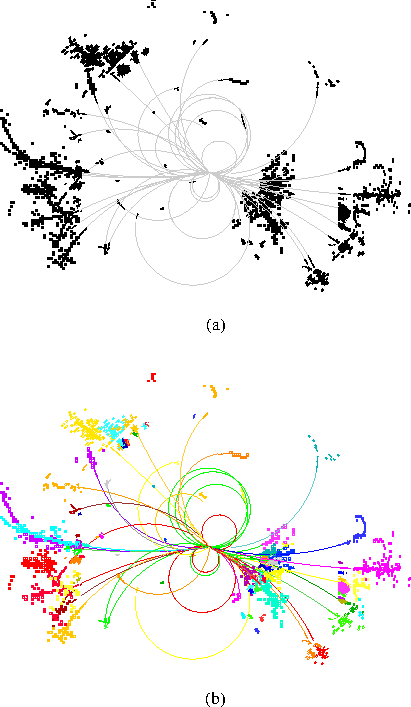
\includegraphics[width=.7\linewidth]{figures/pandora_example.pdf}
    \end{center}
  \end{columns}
\end{frame}

%
% -----------------------------------------------------------------------------
%
\section{Conclusions and Plans}

\begin{frame}
  \frametitle{Conclusion and Plans}

  \bluetext{Future Circular Collider}
  \begin{itemize}
    \item FCC Integrated program is an ambitious CERN project
    \item Feasibility to be proved by the next European HEP Strategy
  \end{itemize}

  \bluetext{Noble Liquid Calorimeters}
  \begin{itemize}
    \item Noble Liquid calorimeter in reference FCC-hh detector, option in
          FCC-ee
    \item Multiple R\&D projects directed at noble liquid  calorimetry at FCC-ee
  \end{itemize}

  \bluetext{Our involvement}
  \begin{itemize}
    \item Performance optimization in the FCC-ee framework
    \item Implement particle flow algorithm for LAr calorimeter
  \end{itemize}

  \begin{center}
    \bluetext{\bf New souls are welcome!}
  \end{center}
\end{frame}

%
% -----------------------------------------------------------------------------
%
\appendix
\backupbegin{}

\begin{frame}[c]
  \begin{center}
    \redtext{\Huge Backup}
  \end{center}
\end{frame}


\begin{frame}
  \frametitle{R\&D FCC-ee LAr Projects}

  CERN EP R\&D projects relevant for Noble Liquid Calorimetry:

  \begin{enumerate}
    \item Read-Out Electrode Design and Performance Optimization
    \item High Density Feed Through Design Investigations
    \item Carbon Composite Cryostats
    \item General SW framework
  \end{enumerate}

  CERN, Charles U. and LAL Orsay: H2020 project AIDAInnova

\end{frame}


\begin{frame}
  \frametitle{Dual Readout Performance}

  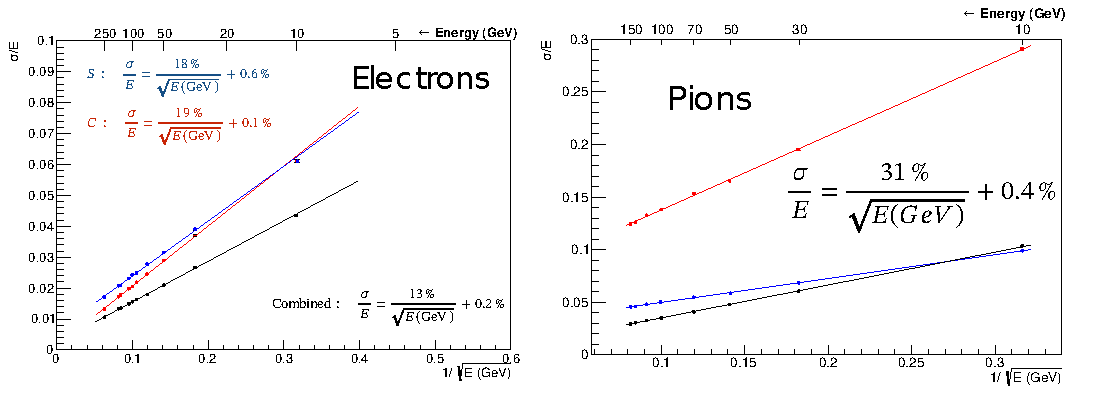
\includegraphics[width=\linewidth]{figures/dual_readout_performance.pdf}
\end{frame}

\begin{frame}
  \frametitle{Crystals Performance}

  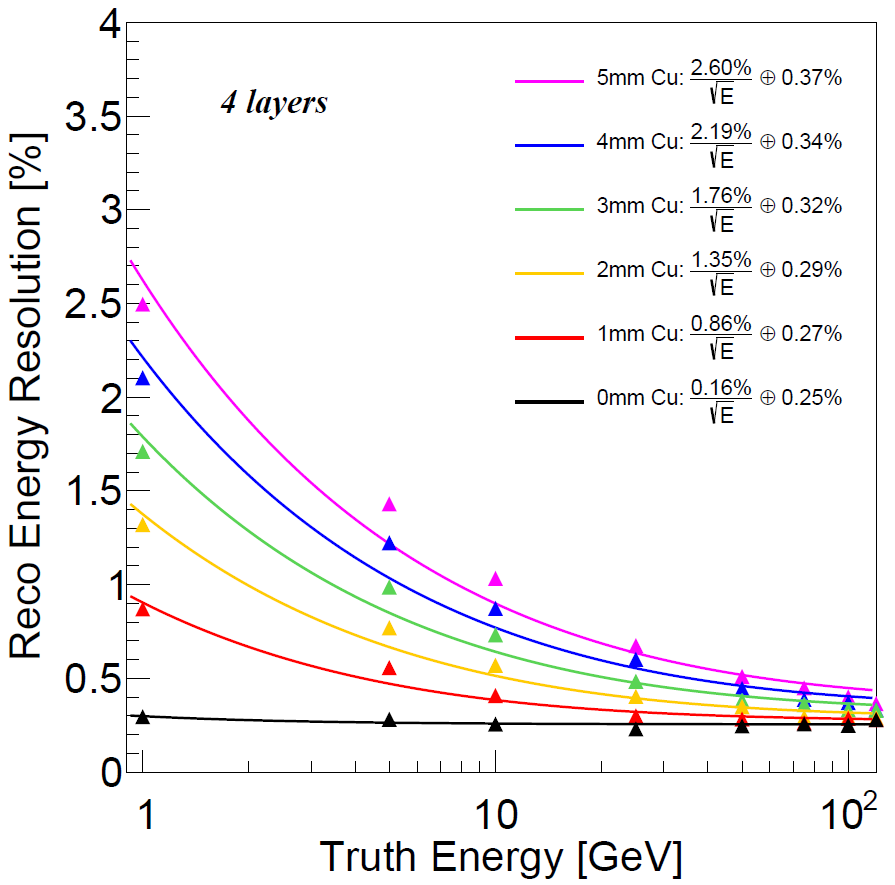
\includegraphics[width=.49\linewidth]{figures/CEPC_crystal_calo_perf_4layers.png}
  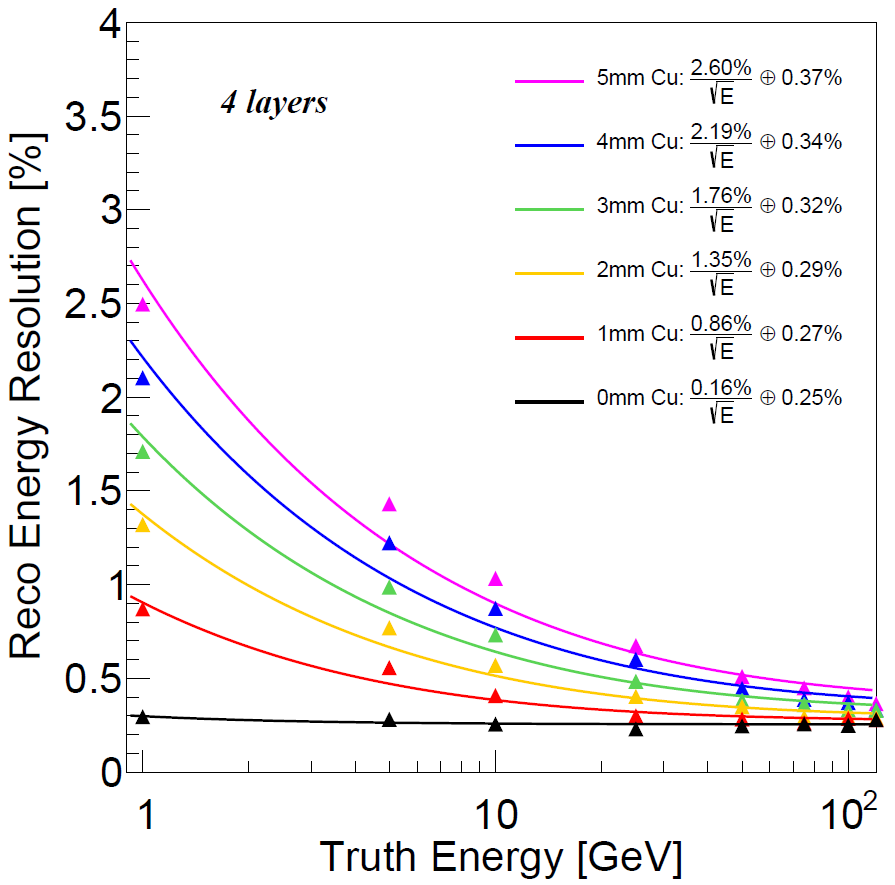
\includegraphics[width=.49\linewidth]{figures/CEPC_crystal_calo_perf_4layers.png}
\end{frame}


\begin{frame}
  \frametitle{FCC-hh: Reference Detector}

  \begin{adjustwidth}{-2em}{-2em}
    \includegraphics[width=\linewidth]{figures/FCC_hh_ref_detector.png}
  \end{adjustwidth}
\end{frame}

\begin{frame}
  \frametitle{FCC-hh: Reference Detector}

  \begin{adjustwidth}{-2em}{-2em}
    \includegraphics[width=\linewidth]{figures/FCC_hh_ref_detector_xsec.pdf}
  \end{adjustwidth}
\end{frame}


\begin{frame}
  \frametitle{FCC and ILC proposal}
  \begin{columns}[c]
    \column{.5\textwidth}
    \begin{center}
      FCC\\
      \includegraphics[width=\linewidth]{figures/fcc-timeline-withILC.png}
    \end{center}
    \column{.5\textwidth}
    \begin{center}
      ILC\\
      \includegraphics[width=\linewidth]{figures/ilc-timeline-withFcc.png}
    \end{center}
  \end{columns}
  \tiny{Image: \href{https://arxiv.org/abs/1912.11871}{arXiv:1912.11871}}\\
\end{frame}

\backupend{}

\end{document}
